% reducesymm/presentations/LesHouch18/finiteQED.tex    pdflatex finiteQED; biber finiteQED
% Predrag 2018-05-30

% if you get        LaTeX Error: Command \block already defined.
%                   l.512 \newcommand{\block}[1]{\ensuremath{#1}}
% press [Enter] once

%  started with siminos/presentations/GTmath18/GTmath18.tex 2018-03-02

% talks/predrag/inputs/layoutBeamer.tex				Predrag 2011.06.17
% $Author: predrag $
% $Date: 2011-11-29 02:19:08 -0500 (Tue, 29 Nov 2011) $

                        %% logical setup, no need to edit %%%%%%%%%%
                        \newif\ifpaper \newif\ifPDF               %%
                        \newif\ifOUP \newif\ifboyscout            %%
                        \newif\ifdasbuch \newif\ifarticle         %%
                        \dasbuchtrue %% DasBuch, not QFT lectures %%
                        \OUPfalse \articlefalse  %% ChaosBook %%%%%%

                        %% uncomment the desired version:
   \paperfalse\PDFtrue  % hyperlinked WWW/chapters/ChaosBook.pdf
%  \papertrue\PDFtrue   % paper B&W pdf for WWW/chapters/
%  \paperfalse\PDFfalse % postscript paper print book.ps, abandoned

%  \boyscouttrue        % commented, for WWW/chapters/boyscouts
   \boyscoutfalse       % public, for WWW/chapters/

\documentclass[compress,hyperref={colorlinks}]{beamer}
%\documentclass{beamer}
%\documentclass{powerdot}
%\documentclass{slides}[14pt]
%\pagestyle{empty}
%\normalsize

\usepackage{etex}		% must be the first after the \documentclass

\usepackage{amsmath}
\usepackage{amssymb}
\usepackage{amscd}
\usepackage{graphicx}
\usepackage{moreverb}
\usepackage[all]{xy}

% Standard packages
\usepackage[english]{babel}
\usepackage[latin1]{inputenc}
\usepackage{times}
\usepackage[T1]{fontenc}

\usepackage{ifthen}         %% used for boolean logic commands

%\usepackage{hyperref} % loaded by beamer already
%\usepackage[pdfauthor={Predrag Cvitanovic'},%
%             pdftitle={finite QED},%
%             colorlinks]{hyperref} %% hyperlinks

%% directories with graphics files
\graphicspath{{../../figs/}{../../Fig/}}

% \usepackage[all]{xy}
% \usepackage{beamerthemesplit}

%% Setup appearance:
% \usetheme{Darmstadt}
% \usetheme{umbc2}
% \usetheme{Boadilla}
\useinnertheme{rounded}
\usecolortheme[RGB={205,173,0}]{structure}
% \usecolortheme{seagull} %dove} %
\setbeamertemplate{items}[ball]
\setbeamertemplate{blocks}[rounded][shadow=true]
\usefonttheme[onlylarge]{structurebold}
\setbeamerfont*{frametitle}{size=\normalsize,series=\bfseries}
\setbeamertemplate{navigation symbols}{}

% \pgfdeclareimage[height=0.5cm]{GTlogo}{GTlogo.png}
% \logo{\pgfuseimage{GTlogo}}

\usepackage[font=scriptsize, labelfont=bf]{caption}
\usepackage[
    backend=biber,  %bibtex,
    sorting=nyt,
    %refsection=chapter,
    %citereset=chapter,
    style=numeric, %alphabetic, % %style=authoryear,
    natbib=true,
    style=phys, % aps
    biblabel= brackets, % superscript, %
    articletitle=false, % true,  % false, % aps
    %chaptertitle=true,  % aip;  % false, % aps
    pageranges = true , % aip: the full range
             % = false, % aps: only the first page being printed
    sortlocale=en_US,
    firstinits=true,
    url=false, %true,  %
    doi=false, %true,
    eprint=false
]{biblatex}
\addbibresource{../../bibtex/QFT.bib}
\setbeamerfont{footnote}{size=\tiny}
% def.tex
% $Author$ $Date$

%%%%%%%%%%%%%%%%%%%%%%%%%%%%%%%%%%%%%%%%%%%%%%%%%%%%%%%%%%%%%%%%%%%%%%%%%
%% defines macros used throughout ChaosBook and related
%%%%%%%%%%%%%%%%%%%%%%%%%%%%%%%%%%%%%%%%%%%%%%%%%%%%%%%%%%%%%%%%%%%%%%%%%

%               Predrag         27feb2012
%               Predrag         17feb2012
%               Predrag          4feb2012
%               Predrag          9oct2009
%               Predrag         12jun2008
%               Predrag         15dec2008
%               Predrag         29oct2005
%               Predrag         13jul2005
%               Predrag         24apr2005
%               Predrag         14feb2005
%               Predrag         22jan2005
%               Predrag         16nov2004
%               Predrag         13jun2004
%               Predrag          3may2004
%               Predrag         10apr2004
%               Predrag         21feb2004
%               Predrag          4oct2003
%               Predrag         30aug2003
%               Predrag         20jun2003
%               Predrag         17jan2003
%               Predrag          6dec2002
%               Predrag          7jul2002
%               Predrag         19nov2000
%               Ronnie          23sep2000
% Predrag disabled \basedirectory machine identifier    25aug2000
% Predrag created               30oct1994

\ifpaper % prepare for B&W paper printing:
       \newcommand{\href}[2]{{#2}}  % no hyperref
       \newcommand{\HREF}[2]{{#2}}
       \renewcommand{\color}[1]{}       % B&W
       \newcommand{\wwwcb}[1]{{ChaosBook.org#1}}
       \newcommand{\wwwgt}{{birtracks.eu}}
       \newcommand{\wwwQFT}[1]{{ChaosBook.org/\-Field\-Theory#1}}
       \newcommand{\wwwcnsQFT}[1]{{ChaosBook.org/\-Field\-Theory#1}}
       \newcommand{\weblink}[1]{{#1}}
       \newcommand{\arXiv}[1]{ {arXiv:#1}}
       \newcommand{\mpArc}[1]{{mp\_arc~#1}}
\else % prepare hyperlinked pdf
        \newcommand{\wwwcb}[1]{       % keep homepage flexible:
                  {\href{http://ChaosBook.org#1}
              {ChaosBook.org#1}}}
       \newcommand{\wwwgt}{{\href{http://birtracks.eu}
              {birtracks.eu}}}
       \newcommand{\wwwQFT}[1]{
                  {\href{http://ChaosBook.org/FieldTheory#1}
              {ChaosBook.org/\-Field\-Theory#1}}}
       \newcommand{\wwwcnsQFT}[1]{
                  {\href{http://ChaosBook.org/FieldTheory#1}
              {ChaosBook.org/\-Field\-Theory#1}}}
       \newcommand{\weblink}[1]{{\href{http://#1}{#1}}}
       \newcommand{\HREF}[2]{
              {\href{#1}{#2}}}
       \newcommand{\mpArc}[1]{
              {\href{http://www.ma.utexas.edu/mp_arc-bin/mpa?yn=#1}
                   {mp\_arc~#1}}}
       \newcommand{\arXiv}[1]{
              {\href{http://arXiv.org/abs/#1}{arXiv:#1}}}
\fi

%%%%%%%%%%%%%%%%%%%%%% QUOTATIONS %%%%%%%%%%%%%%%%%%%%%%%%%%%%%%%%%%%%%%
%
%  the learned/witty quotes at the chapter and section headings
%
\newsavebox{\bartName}
\newcommand{\bauthor}[1]{\sbox{\bartName}{\parbox{\textwidth}{\vspace*{0.8ex}
       %\hspace*{\fill}
       \hspace{2em}---\small\noindent #1}}}
\newenvironment{bartlett}{\hfill\begin{minipage}[t]{0.65\textwidth}\small}%
{\hspace*{\fill}\nolinebreak[1]\usebox{\bartName}\vspace*{1ex}\end{minipage}}
%
%  a quotation inserted into the text
%
\newenvironment{txtquote}{\begin{quotation} \small}{\end{quotation}}

\newcommand{\student}{Henriette Roux}
%\newcommand{\student}{Jens J. Jensen}

%%%%%%%%%%%%%%%%%%%%%% INDEXING %%%%%%%%%%%%%%%%%%%%%%%%%%%%%%%%%%%%%%%%%
\newcommand{\indx}[1] {#1\index{#1}}    % do not need to repeat the word

\newcommand{\file}[1]{$\footnotemark\footnotetext{{\bf file} #1}$}
% PC 9sep2008 commented out (is it used?):
%\newcommand{\lecture}[2]{ \addtocontents{toc}
%           {{\scriptsize #1}{\sf\small lecture: \scriptsize #2}} }

%%%%%%%%%%%%%%% EQUATIONS %%%%%%%%%%%%%%%%%%%%%%%%%%%%%%%
\newcommand{\beq}{\begin{equation}}
\newcommand{\continue}{\nonumber \\ }
\newcommand{\nnu}{\nonumber}
\newcommand{\eeq}{\end{equation}}
\newcommand{\ee}[1] {\label{#1} \end{equation}}
\newcommand{\bea}{\begin{eqnarray}}
\newcommand{\ceq}{\nonumber \\ & & }
\newcommand{\eea}{\end{eqnarray}}
\newcommand{\barr}{\begin{array}}
\newcommand{\earr}{\end{array}}

%%%%%%%%%%%%%%% REFERENCING EQUATIONS ETC. %%%%%%%%%%%%%%%%%%%%%%%%%%%%%%%
\newcommand{\rf}     [1] {~\cite{#1}}
\newcommand{\refref} [1] {ref.~\cite{#1}}
\newcommand{\refRef} [1] {Ref.~\cite{#1}}
\newcommand{\refrefs}[1] {refs.~\cite{#1}}
\newcommand{\refRefs}[1] {Refs.~\cite{#1}}
\newcommand{\refeq}  [1] {(\ref{#1})}
\newcommand{\refeqs} [2]{(\ref{#1}--\ref{#2})}
\newcommand{\refpage}[1] {page~\pageref{#1}}
\newcommand{\reffig} [1] {figure~\ref{#1}}
\newcommand{\reffigs} [2] {figures~\ref{#1} and~\ref{#2}}
\newcommand{\refFig} [1] {Figure~\ref{#1}}
\newcommand{\refFigs} [2] {Figures~\ref{#1} and~\ref{#2}}
\newcommand{\reftab} [1] {table~\ref{#1}}
\newcommand{\refTab} [1] {Table~\ref{#1}}
\newcommand{\reftabs}[2] {tables~\ref{#1} and~\ref{#2}}
\newcommand{\refsect}[1] {sect.~\ref{#1}}
\newcommand{\refsects}[2] {sects.~\ref{#1} and \ref{#2}}
\newcommand{\refSect}[1] {Sect.~\ref{#1}}
\newcommand{\refSects}[2] {Sects.~\ref{#1} and \ref{#2}}
\newcommand{\refsecttosect}[2] {Sects.~\ref{#1} to~\ref{#2}}
\newcommand{\refchap}[1] {chapter~\ref{#1}}
\newcommand{\refChap}[1] {Chapter~\ref{#1}}
\newcommand{\refchaps}[2] {chapters~\ref{#1} and~\ref{#2}}
\newcommand{\refchaptochap}[2] {chapters~\ref{#1} to~\ref{#2}}
\newcommand{\refappe}[1] {appendix~\ref{#1}}
\newcommand{\refappes}[2] {appendices~\ref{#1} and~\ref{#2}}
\newcommand{\refAppe}[1] {Appendix~\ref{#1}}
\newcommand{\refrem} [1] {remark~\ref{#1}}
\newcommand{\refexam}[1] {example~\ref{#1}}
\newcommand{\refExam}[1] {Example~\ref{#1}}
\newcommand{\refexer}[1] {exercise~\ref{#1}}
\newcommand{\refExer}[1] {Exercise~\ref{#1}}
\newcommand{\refsolu}[1] {solution~\ref{#1}}
\newcommand{\refSolu}[1] {Solution~\ref{#1}}

%%%%%%%%%%%%%%  Abbreviations %%%%%%%%%%%%%%%%%%%%%%%%%%%%%%%%%%%%%%%%
%%% APS (American Physiology Society, it seems) style:
%%%     Latin or foreign words or phrases should be roman, not italic.
%%%     Insert a `hard' space after full points
%%%                                         that do not end sentences.

\newcommand{\etc}{{etc.}}       % APS
\newcommand{\etal}{{\em et al.}}    % etal in italics, APS too
\newcommand{\ie}{{i.e.}}        % APS
\newcommand{\cf}{{\em cf.\ }}     % APS
\newcommand{\eg}{{e.g.\ }}        % APS, OUP, hard space '\eg\ NextWord'
% \newcommand{\etc}{{\em etc.}}     % etcetera in italics
% \newcommand{\ie}{{that is}}       % use Latin or English?  Decide later.
% \newcommand{\cf}{{cf.}}
% \newcommand{\eg}{{\it e.g.,\ }}   % Wirzba 2sep2001

%%%%%%%%%%%%%%% ChaosBook Abbreviations %%%%%%%%%%%%%%%%%%%%%%%%

\newcommand{\evOper}{evolution oper\-ator}
\newcommand{\EvOper}{Evolution oper\-ator}
 %% \newcommand{\evOp}{Ruelle operator} %could be ``evolution'' instead?
%\newcommand{\FPoper}{Frobenius-Perron oper\-ator}
\newcommand{\FPoper}{Perron-Frobenius oper\-ator} % Pesin's ordering
\newcommand{\FP}{Perron-Frobenius}
\newcommand{\statesp}{state space}
\newcommand{\Statesp}{State space}
\newcommand{\fixedpnt}{fixed point}
\newcommand{\Fixedpnt}{fixed point}
\newcommand{\maslov}{topological}
\newcommand{\Maslov}{Topological}
%\newcommand{\Maslov}{Keller-Maslov}
\newcommand{\jacobian}{Jacobian}        % determinant
% \newcommand{\jacobianM}{fundamental matrix} % no known standard name?
% \newcommand{\jacobianMs}{fundamental matrices}  %
% \newcommand{\JacobianM}{Fundamental matrix} %
% \newcommand{\JacobianMs}{Fundamental matrices}  %
\newcommand{\jacobianM}{Jacobian matrix}  % back to Predrag's name 20oct2009
\newcommand{\jacobianMs}{Jacobian matrices}   % matrices
\newcommand{\JacobianM}{Jacobian matrix} %
\newcommand{\JacobianMs}{Jacobian matrices}  %
\newcommand{\FloquetM}{Floquet matrix} % specialized to periodic orb
\newcommand{\FloquetMs}{Floquet matrices}  %
% \newcommand{\stabmat}{matrix of variations}   % Arnold, says Vattay
\newcommand{\stabmat}{stability matrix}     % stability matrix, velocity gradients
\newcommand{\Stabmat}{Stability matrix}     % Stability matrix
\newcommand{\stabmats}{stability matrices}
\newcommand{\monodromyM}{monodromy matrix} % monodromy matrix, Poincare cut
\newcommand{\MonodromyM}{Monodromy matrix} % monodromy matrix, Poincare cut
\newcommand{\dzeta}{dyn\-am\-ic\-al zeta func\-tion}
\newcommand{\Dzeta}{Dyn\-am\-ic\-al zeta func\-tion}
\newcommand{\tzeta}{top\-o\-lo\-gi\-cal zeta func\-tion}
\newcommand{\Tzeta}{Top\-o\-lo\-gi\-cal zeta func\-tion}
\newcommand{\BERzeta}{BER zeta func\-tion}
%\newcommand{\tzeta}{Artin-Mazur zeta func\-tion} %alternative to topological
\newcommand{\qS}{semi\-classical zeta func\-tion}
%\newcommand{\qS}{Gutz\-willer-Voros zeta func\-tion}
\newcommand{\Gt}{Gutz\-willer trace formula}
\newcommand{\Fd}{spec\-tral det\-er\-min\-ant}
%\newcommand{\fd}{spec\-tral det\-er\-min\-ant} %in many articles
\newcommand{\FD}{Spec\-tral det\-er\-min\-ant}
\newcommand{\cFd}{semiclass\-ic\-al spec\-tral det\-er\-mi\-nant}
\newcommand{\cFD}{Semiclass\-ic\-al spec\-tral det\-er\-mi\-nant}
% \newcommand{\cFd}{semiclass\-ic\-al Fred\-holm det\-er\-mi\-nant}
\newcommand{\Vd}{Vattay det\-er\-mi\-nant}
\newcommand{\cycForm}{cycle averaging formula}
\newcommand{\CycForm}{Cycle averaging formula}
\newcommand{\freeFlight}{mean free flight time}
\newcommand{\FreeFlight}{Mean free flight time}
\newcommand{\pdes}{partial differential equations}
\newcommand{\Pdes}{Partial differential equations}
\newcommand{\dof}{dof}         % Hamiltonian deegree of freedom
% \newcommand{\dof}{deegree of freedom}

%%%%%%%%%%%%%%% VECTORS, MATRICES, NORMS %%%%%%%%%%%%%%%%%%%%%%%%%%%%%%%%%

	% without large brackets:
\newcommand{\braket}[2]
		   {\langle{#1}\vphantom{#2}|\vphantom{#1}{#2}\rangle}
\newcommand{\bra}[1]{\langle{#1}\vphantom{ }|}
\newcommand{\ket}[1]{|\vphantom{}{#1}\rangle}
	% with large brackets:
%\newcommand{\bra}[1]{\left\langle{#1}\vphantom{ }\right|}
%\newcommand{\ket}[1]{\left|\vphantom{}{#1}\right\rangle}
%\newcommand{\braket}[2]{\left\langle{#1}
%                        \vphantom{#2}\right|\left.\vphantom{#1}
%                        {#2}\right\rangle}

\newcommand{\dual}[1]{{#1}^\ast}
% \newcommand{\transp}[1]{\bar{#1}}
\newcommand{\transp}[1]{{#1}{}^\top}

% Commented out AMS-style pmatrix, which is incompatible with TeX/LaTeX pmatrix
% used throughout dasbuch. Fri Oct 12 15:51:03 EDT 2007

\newcommand{\MatrixII}[4]{\left(
\begin{array}{cc}
{#1}  &  {#2} \\
{#3}  &  {#4} \end{array} \right)}
% a problem with \pmatrix 12oct 2007
%\newcommand{\MatrixII}[4]{
%   \begin{pmatrix}{#1}  &  {#2} \\
%                  {#3}  &  {#4} \end{pmatrix}}

\newcommand{\MatrixIII}[9]{
  \pmatrix{ {#1}  &  {#2} &  {#3} \cr
            {#4}  &  {#5} &  {#6} \cr
            {#7}  &  {#8} &  {#9}
          }               }
% \newcommand{\MatrixIII}[9]{
%    \begin{pmatrix} {#1}  &  {#2} &  {#3} \\
%                    {#4}  &  {#5} &  {#6} \\
%                    {#7}  &  {#8} &  {#9}  \end{pmatrix}}


% \newcommand{\transpVectorII}[2]{
%    \begin{pmatrix}{#1}  &  {#2}  \end{pmatrix}}

\newcommand{\VectorII}[2]{\left(
\begin{array}{cc}
{#1}  &  {#2} \end{array} \right)}
%
%\newcommand{\VectorII}[2]{
%  \pmatrix{ {#1} \cr {#2}}
%}

% \newcommand{\VectorII}[2]{
%    \begin{pmatrix} {#1} \\
%                    {#2}  \end{pmatrix}}

% \newcommand{\VectorIII}[3]{
%    \begin{pmatrix} {#1} \\
%                    {#2} \\
%                    {#3} \end{pmatrix}}

\newcommand{\transpVectorII}[2]{
  \pmatrix{ {#1}  &  {#2}}
}

\newcommand{\VectorIII}[3]{
  \pmatrix{ {#1} \cr
            {#2} \cr
            {#3}
          }
}

\newcommand{\combinatorial}[2]{ {#1 \choose #2}}

%%%%%%%%%%%%%%% Sundry symbols within math eviron.: %%%%%%%%%%%%

\newcommand{\obser}{\ensuremath{a}}     % an observable from phase space to R^n
\newcommand{\Obser}{\ensuremath{A}}     % time integral of an observable
\newcommand{\onefun}{\iota} % the function that returns one no matter what
\newcommand{\defeq}{=}      % the different equal for a definition
\newcommand {\deff}{\stackrel{\rm def}{=}}
\newcommand{\reals}{\mathbb{R}}
\newcommand{\complex}{\mathbb{C}}
\newcommand{\integers}{\mathbb{Z}}
\newcommand{\rationals}{\mathbb{Q}}
\newcommand{\naturals}{\mathbb{N}}
\newcommand{\LieD}{{{\cal L}\!\!\llap{-}\,\,}}  % {{\pound}} % Lie Derivative
\newcommand{\half}{{\scriptstyle{\frac{1}{2}}}}
\newcommand{\pde}{\partial}
\newcommand{\pdfrac}[2]{\frac{\partial #1}{\partial #2}}
\renewcommand\Im{\ensuremath{{\rm Im}\,}}
\renewcommand\Re{\ensuremath{{\rm Re}\,}}
\renewcommand{\det}{\mbox{\rm det}\,}
\newcommand{\Det}{\mbox{\rm Det}\,}
\newcommand{\tr}{\mbox{\rm tr}\,}
\newcommand{\Tr}{\mbox{\rm tr}\,}
%\newcommand{\Tr}{\mbox{Tr}\,}
\newcommand{\sign}[1]{\sigma_{#1}}
%\newcommand{\sign}[1]{{\rm sign}(#1)}
\newcommand{\mInv}{{I}}                 % material invariant
\newcommand{\msr}{\ensuremath{\rho}}                % measure
\newcommand{\Msr}{{\mu}}                % coarse measure
\newcommand{\dMsr}{{d\mu}}              % measure infinitesimal
\newcommand{\SRB}{{\rho_0}}             % natural measure
\newcommand{\vol}{{V}}                  % volume of i-th tile
\newcommand{\prpgtr}[1]{\delta\negthinspace\left( {#1} \right)}
%\newcommand{\Zqm}{\ensuremath{Z_{qm}}}         % Gutz-Voros zeta function
\newcommand{\Zqm}{\ensuremath{\det(\hat{H} - E)_{sc} }} % semicls spectr. det:
\newcommand{\Fqm}{\ensuremath{F_{qm}}}
\newcommand{\zfct}[1]{\zeta ^{-1}_{#1}}
\newcommand{\zetaInv}{\ensuremath{1/\zeta}}
% \newcommand{\zetaInv}{{\zeta^{-1}}}
\newcommand{\zetatop}{\ensuremath{1/\zeta_{\mbox{\footnotesize top}} }}
\newcommand{\zetaInvBER}[1]{1/\zeta_{\mbox{\footnotesize BER}}(#1)}
\newcommand{\BER}[1]{{\mbox{\footnotesize BER}}} % Baladi-Ruelle-Eckmann
\newcommand{\eigCond}{\ensuremath{F}}           % eigenvalue cond. function
\newcommand{\expct}    [1]{\left\langle {#1} \right\rangle}
\newcommand{\spaceAver}[1]{\left\langle {#1} \right\rangle}
\newcommand{\timeAver} [1]{\overline{#1}}
\newcommand{\norm}[1]{\left\Arrowvert \, #1 \, \right\Arrowvert}
\newcommand{\pS}{\ensuremath{{\cal M}}}          % symbol for state space
\newcommand{\ssp}{\ensuremath{x}}                % state space point
\newcommand{\tissp}{\tilde{\Delta\ssp}} % Rytis \CostFct
\newcommand{\pSpace}{x}       % Hamiltonian phase space x=(q,p) coordinate
\newcommand{\coord}{q}        % configuration space p coordinate
\newcommand{\DOF}{\ensuremath{D}}          % Hamiltonian deegree of freedom
\newcommand{\NWS}{\ensuremath{\Omega}}     % symbol for the non--wandering set
\newcommand{\AdmItnr}{\Sigma}      % set of admissible itineraries
\newcommand{\intM}[1]{{\int_\pS{\!d #1}\:}} %phase space integral
\newcommand{\Cint}[1]{\oint\frac{d#1}{2 \pi i}\;} %Cauchy contour integral
\newcommand{\PoincS}{\ensuremath{{\cal P}}}  % symbol for Poincare section
\newcommand{\PoincM}{\ensuremath{P}}       % symbol for Poincare map
\newcommand{\PoincC}{\ensuremath{U}}       % symbol for Poincare constraint function
\newcommand{\arc}{\ensuremath{s}}          % symbol for billiard wall arc
\newcommand{\mompar}{\ensuremath{p}}       % billiard wall parall. momentum
\newcommand{\restCoeff}{\ensuremath{\gamma}}  % billiard wall restitution coeff
\newcommand{\timeIn}[1]{{t^{-}_{#1}}} % billiard wall time of arrival
\newcommand{\timeOut}[1]{{t^{+}_{#1}}}   % billiard wall time of departure
%\newcommand{\PoincS}{\partial{\cal M}}          % billiard Poincare section
\newcommand{\Lop}{\ensuremath{{\cal L}}}       % evolution operator
\newcommand{\Uop}{\ensuremath{{\cal K}}}       % Koopman operator, Driebe notation
%\newcommand{\Uop}{\ensuremath{{\cal L}^\dagger}}  % Koopman, adjoint notation
\newcommand{\Aop}{\ensuremath{{\cal A}}}       % evolution generator
\newcommand{\TrOp}{\ensuremath{{\cal T}}}       % transfer operator, like in statmech
\newcommand{\matId}{\ensuremath{{\bf 1}}}      % matrix identity
\newcommand{\eigenvL}{\ensuremath{s}}      % evolution operator eigenvalue
\newcommand{\eigenvG}{\ensuremath{m}}      % compact group eigenvalues
\newcommand{\inFix}[1]{{\in \mbox{\footnotesize Fix}f^{#1}}}
\newcommand{\inZero}[1]{{\in \mbox{\footnotesize Zero} \, f^{#1} }}
\newcommand{\xzero}[1]{{x_{#1}^\ast}}
\newcommand{\fractal}{{{\cal F}}}
\newcommand{\contract}{F}
% \newcommand{\presentation}{P} % PC commented out 7sep2008
\newcommand{\orderof}[1]{o(#1)} % Rytis 22mar2005

     %%%%%%%%%% flows: %%%%%%%%%%%%%%%%%%%%%%%%%%%%
\newcommand\map{f}                  % other people like \phi's etc
\newcommand\flow[2]{{f^{#1}(#2)}}
\newcommand{\vel}{\ensuremath{v}}   % state space velocity
\newcommand\velField[1]{{v(#1)}}    % ODE velocity field
\newcommand\invFlow{F}
\newcommand\hflow[2]{{\hat{f}^{#1}(#2)}}
\newcommand\timeflow{{f^t}}
\newcommand\tflow[2]{{\tilde{f}^{#1}(#2)}}
%\newcommand\tflow{\tilde{f}^\tau}        %RECHECK USE OF THIS!
\newcommand\xInit{{x_0}}        %initial x
%\newcommand\xInit{\xi}     %initial x, Spiegel notation
\newcommand{\para}{\parallel}
\newcommand\multiX{x}       %multi point n-dim vector
\newcommand\multiF{f}       %multi point n-dim vector mapping

   %%%%%%% 3D physical flow
\newcommand{\stagp}{stagnation point}
\newcommand{\Stagp}{Stagnation point}
\newcommand{\relstagp}{traveling stagnation point}
\newcommand{\Relstagp}{Traveling stagnation point}
\newcommand{\velgradmat}{velocity gradients matrix}

   %%%%%%%% Siminos thesis %%%%%%%%%%%%%%%%%%%%%%%%%%%%
\newcommand{\Le}{Lorenz equations}
\newcommand{\rLor}{\rho}    % parameter r in Lorenz paper
\newcommand{\cLe}{complex Lorenz equations}
\newcommand{\cLf}{complex Lorenz flow}
\newcommand{\CLe}{Complex Lorenz equations}
\newcommand{\CLf}{Complex Lorenz flow}
\newcommand{\RerCLor}{\rho_1}    % real      part of parameter r, CLe
\newcommand{\ImrCLor}{\rho_2}    % imaginary part of parameter r, CLe
% \newcommand{\AGHe}{Armbruster-Guckenheimer-Holmes flow}

     %%%%%%%%%% periods: %%%%%%%%%%%%%%%%%%%%%%%%%%%%
\newcommand\period[1]{{\ensuremath{T_{#1}}}}         %continuous cycle period
%\newcommand\period[1]{{\tau_{#1}}}
\newcommand{\cl}[1]{{\ensuremath{n_{#1}}}}   % discrete length of a cycle, Predrag
%\newcommand{\cl}[1]{|#1|}  % the length of a periodic orbit, Ronnie
\newcommand{\nCutoff}{N}    % maximal cycle length
                % maximal stability cutoff:
\newcommand{\stabCutoff}{\ExpaEig_{\mbox{\footnotesize max}}}
\newcommand{\timeSegm}[1]{{\tau_{#1}}}      %billiard segment time period
\newcommand{\timeStep}{\ensuremath{{\delta \tau}}}  %integration step
\newcommand{\deltaX}{\ensuremath{{\delta x}}}       %trajectory displacement
\newcommand{\unitVec}{\ensuremath{\hat{n}}}     %unit vector

\newcommand{\Mvar}{\ensuremath{A}}  % stability matrix
\newcommand{\derF}[1]{\ensuremath{A(#1)}}   % Predrag stability matrix
 %\newcommand{\derF}[1]{{DF |_{#1}}}        % Gibson stability matrix
\newcommand{\jMps}{\ensuremath{J}}   % jacobian matrix, phase space/state space
% \newcommand{\jMps}{\ensuremath{{\bf J}}}  % bold fundamental matrix phase space
\newcommand{\derf}[2]{\ensuremath{{J}^{#1}(#2)}}    % Predrag fundamental matrix
% \newcommand{\derf}[2]{\ensuremath{{\bf J}^{#1}(#2)}}  % Predrag bold fundamental matrix
 % \newcommand{\derf}[2]{{Df^{#1}|_{#2}}}   % Gibson fundamental matrix
\newcommand{\jMConfig}{\ensuremath{{\bf j}}}    % fundamental matrix, configuration space
\newcommand{\jConfig}{\ensuremath{j}}      % jacobian, configuration space
\newcommand{\jMP}{\ensuremath{\hat{J}}}   % jacobian matrix, Poincare return
% \newcommand{\jMP}{\ensuremath{{\bf \hat{J}}}}   % bold jacobian matrix, Poincare return
\newcommand{\monodromy}{\ensuremath{M}}   % monodromy matrix, full Poincare cut
% \newcommand{\monodromy}{\ensuremath{{\bf M}}}   % bold monodromy matrix, full Poincare cut
                   % Fredholm det jacobian weight:
%\newcommand{\jEigvec}[1]{\ensuremath{{\bf e}^{(#1)}}}  % right jacobiam eigenvector
%\newcommand{\jEigvecT}[1]{\ensuremath{{\bf e}_{(#1)}}}  % left jacobiam eigenvector
\newcommand{\jEigvec}[1][]{\ensuremath{{\bf e}^{(#1)}}} % right jacobiam eigenvector
\newcommand{\jEigvecT}[1][]{\ensuremath{{\bf e}_{(#1)}}} % left jacobiam eigenvector
\newcommand{\oneMinJ}[1]
           {\left|\det\!\left(\matId-\monodromy_p^{#1}\right)\right|}
\newcommand{\maslovInd}{\ensuremath{m}}        % Maslov index
\newcommand{\ExpaEig}{\ensuremath{\Lambda}}
\newcommand{\Lyap}{\ensuremath{\lambda}}            %Lyapunov exponent

%%   optional parameter comes in [\ldots], for example
%%   \newcommand\eigRe[1][ ]{\ensuremath{\mu_{#1}}}
%%   no subscript: \eigRe\
%%   with subscript j: \eigRe[j]
%%
% \newcommand{\eigExp}[1][ ]{\ensuremath{\lambda_{#1}}}   % complex eigenexponent
%%  Guckenheimer&Holmes:  lambda = alpha + i beta
%%  Hirsch-Smale:         lambda = a     + i b
%%  Boyce-di Prima:       lambda = mu    + i nu
% \newcommand{\eigRe}[1][ ]{\ensuremath{\mu_{#1}}}    % Re eigenexponent
% \newcommand{\eigIm}[1][ ]{\ensuremath{\nu_{#1}}}    % Im eigenexponent

\newcommand{\eigExp}[1][]{
     \ifthenelse{\equal{#1}{}}{\ensuremath{\lambda}}{\ensuremath{\lambda^{(#1)}}}}
\newcommand{\eigRe}[1][]{
     \ifthenelse{\equal{#1}{}}{\ensuremath{\mu}}{\ensuremath{\mu^{(#1)}}}}
\newcommand{\eigIm}[1][]{
     \ifthenelse{\equal{#1}{}}{\ensuremath{\omega}}{\ensuremath{\omega^{(#1)}}}}

\newcommand\LyapTime{T_{\mbox{\footnotesize Lyap}}} %Lyapunov time
\newcommand{\hatx}{{\hat{x}}}
% \newcommand{\hatx}{{\hat{x}_t}}               %RECHECK USE OF THIS!
\newcommand{\hatp}{{\hat{x}_p}}
\newcommand{\phat}{{\hat{p}}}
\newcommand{\curvR}{\rho}           %billiard curvature
\newcommand{\dz}{{\delta z}}
\newcommand{\dth}{{\delta \theta}}
\newcommand{\delh}{{\delta h}}
\newcommand{\NN}{{{\cal N}}}

%%%%%%%%%%%%%%% symbolic dynamics %%%%%%%%%%%%%%%%%%%%%%%%%%%%%%%%%%
\newcommand{\MarkGraph}{Transition graph} % following Yorke
\newcommand{\markGraph}{transition graph} % following Yorke
% \newcommand{\MarkGraph}{Markov graph}
\newcommand{\admissible}{admissible}
\newcommand{\Admissible}{Admissible}
\newcommand{\inadmissible}{inadmissible}
\newcommand{\cycle}[1]{{\ensuremath{\overline{#1}}}}
\newcommand{\cycpt}{_{p,m}}
\newcommand\sumprime{\mathop{{\sum}'}}
\newcommand{\pseudos}{\pi}
% \newcommand{\pseudos}{{p_1+p_2+\dots+p_k}}
% \newcommand{\pseudos}{{\{p_1 p_2 \dots p_k\}}}
\newcommand{\block}[1]{\ensuremath{#1}} % PC 07sep2008: conflict with beamer
\newcommand{\prune}[1]{\ensuremath{\_{#1}\_}}        % fits into math env.
%\newcommand{\prune}[1]{\ldots{#1}\ldots}
%\newcommand{\strng}[1]{$\_#1\_$}    % fits into text without $'s
% replaced \strng by \prune throughout
\newcommand{\biinf}[2]{\ensuremath{\cdots#1.#2\cdots}}
\newcommand{\rctngl}[2]{\ensuremath{[#1.#2]}}
\newcommand{\BKsym}[1]{\ensuremath{S_{#1}}}
\newcommand{\Ksym}[1]{{\ensuremath{\sigma_{#1}}}}
\newcommand{\Ssym}[1]{{\ensuremath{s_{#1}}}}
\newcommand{\gmax}{\ensuremath{\hat{\gamma}}}
\newcommand{\Spast}{\ensuremath{S^\textrm{-}}}       % past itenerary
\newcommand{\Sfuture}{\ensuremath{S^\textrm{\scriptsize +}}} % future itenerary
\newcommand{\Sbiinf}{\ensuremath{S}}             % biinf. itenerary
\newcommand{\str}{\ensuremath{\epsilon_{1},\epsilon_{2}, \ldots} } % Ronnie's problems

%%%%%%%%%%%%%%% relative periodic orbits: %%%%%%%%%%%%%%%%%%%%%%%%%%%%
\newcommand{\po}{periodic orbit}
\newcommand{\Po}{Periodic orbit}
\newcommand{\rpo}{rela\-ti\-ve periodic orbit}
%   \newcommand{\rpo}{equi\-vari\-ant periodic orbit}
\newcommand{\Rpo}{Rela\-ti\-ve periodic orbit}
%   \newcommand{\Rpo}{Equi\-vari\-ant periodic orbit}
\newcommand{\eqv}{equi\-lib\-rium}
\newcommand{\Eqv}{Equi\-lib\-rium}
\newcommand{\eqva}{equi\-lib\-ria}
\newcommand{\Eqva}{Equi\-lib\-ria}
\newcommand{\reqv}{rela\-ti\-ve equi\-lib\-rium}
%   \newcommand{\reqv}{equi\-vari\-ant equilibrium}
%   \newcommand{\reqv}{travelling wave}
\newcommand{\Reqv}{Rela\-ti\-ve equi\-lib\-rium}
%   \newcommand{\Reqv}{Equi\-variant equi\-librium}
%   \newcommand{\Reqv}{travelling wave}
\newcommand{\reqva}{rela\-ti\-ve equi\-lib\-ria}
%   \newcommand{\reqva}{equivariant equilibria}
\newcommand{\Reqva}{Rela\-ti\-ve equi\-lib\-ria}
%   \newcommand{\Reqva}{Equivariant equilibria}
\newcommand{\equilibrium}{equi\-lib\-rium}
\newcommand{\equilibria}{equi\-lib\-ria}
\newcommand{\Equilibria}{Equi\-lib\-ria}
% \newcommand{\equilibrium}{steady state}
% \newcommand{\equilibria}{steady states}
% \newcommand{\Equilibria}{Steady states}
\newcommand{\Hec}{Hetero\-clinic connect\-ion}
\newcommand{\hec}{hetero\-clinic connect\-ion}
\newcommand{\HeC}{Hetero\-clinic Connect\-ion}

%%%%%%%%%%%%%%% SECTIONS, SLICES %%%%%%%%%%%%%%%%%%%%%%%%%%%%%%%%%

\newcommand{\Poincare}{Poincar\'e }
\newcommand{\PoincSec}{Poincar\'e section}
% \newcommand{\reducedsp}{orbit space}
% \newcommand{\Reducedsp}{Orbit space}
\newcommand{\reducedsp}{reduced state space}
\newcommand{\Reducedsp}{Reduced state space}
\newcommand{\fixedsp}{fixed-point subspace}
\newcommand{\Fixedsp}{Fixed-point subspace}
\newcommand{\csection}{cross-section} % eventually eliminate
\newcommand{\Csection}{Cross-section} % eventually eliminate
\newcommand{\slice}{slice}
\newcommand{\Slice}{Slice}
\newcommand{\mslices}{method of slices}
\newcommand{\Mslices}{Method of slices}
\newcommand{\mframes}{method of moving frames}
\newcommand{\Mframes}{Method of moving frames}
\newcommand{\chartBord}{chart border}
\newcommand{\ChartBord}{Chart border}
\newcommand{\poincBord}{section border}
\newcommand{\PoincBord}{Section border}
% \newcommand{\poincBord}{\PoincSec\ border}
% \newcommand{\PoincBord}{\PoincSec\ border}
% \newcommand{\poincBord}{border of transversality}
\newcommand{\template}{template} % {slice-fixing point} % {reference state}
\newcommand{\sliceBord}{slice border}
\newcommand{\SliceBord}{Slice border}
\newcommand{\Sset}{Inflection hyperplane}
\newcommand{\sset}{inflection hyperplane} 	% {singularity hyperplane}
											% {singular set}
\newcommand{\pSRed}{\ensuremath{\hat{\cal M}}} % reduced state space Jan 2012
%\newcommand{\pSRed}{\ensuremath{\bar{\cal M}}} % reduced state space
\newcommand{\sspRed}{\ensuremath{\hat{\ssp}}}    % reduced state space point Jan 2012
% \newcommand{\sspRed}{\ensuremath{y}}    % reduced state space point, experiment
% \newcommand{\sspRed}{\ensuremath{\bar{x}}}    % reduced state space point
\newcommand{\velRed}{\ensuremath{\hat{\vel}}}    % ES reduced state space velocity Jan 2012
% \newcommand{\velRed}{\ensuremath{\bar{v}}}    % PC reduced state space velocity
% \newcommand{\velRed}{\ensuremath{u}}    % ES reduced state space velocity

\newcommand{\slicep}{{\ensuremath{\sspRed'}}}   % slice-fixing point Jan 2012
% \newcommand{\slicep}{{\ensuremath{y'}}}   % slice-fixing point, experimental
% \newcommand{\slicep}{\ensuremath{\ssp'}}   % slice-fixing point
%\newcommand{\sliceTan}[1]{\ensuremath{t_{#1}(y')}}    % tangent at slice-fixing, experimental
\newcommand{\sliceTan}[1]{\ensuremath{t'_{#1}}}    % group orbit tangent at slice-fixing
\newcommand{\groupTan}{\ensuremath{t}}    % group orbit tangent
%\newcommand{\Group}{\ensuremath{\Gamma}}    % Siminos Lie group
\newcommand{\Group}{\ensuremath{G}}         % Predrag Lie or discrete group
%\newcommand{\Lg}{\mathfrak{a}}             % Siminos Lie algebra generator
\newcommand{\Lg}{\ensuremath{\mathbf{T}}}   % Predrag Lie algebra generator
%\newcommand{\LieEl}{\ensuremath{\mathbb{G}}}  % Wiczek project Lie group element
\newcommand{\LieEl}{\ensuremath{g}}  % Predrag Lie group element

\newcommand{\zeit}{\ensuremath{t}}  %time variable Ashley
\newcommand{\sspSing}{\ensuremath{\ssp^\ast}} 	% inflection point
\newcommand{\sspRSing}{\ensuremath{\sspRed^\ast}} 	% inflection point, reduced space

%%%%%%%%%%%%%%% LIE GROUP PARAMETRIZATIONS %%%%%%%%%%%%%%%%%%%%%%
\newcommand{\gSpace}{\ensuremath{{\bf \phi}}}   % MA group rotation parameters
% \newcommand{\gSpace}{\ensuremath{{\bf \theta}}}   % PC group rotation parameters
\newcommand{\velRel}{\ensuremath{c}}    % relative state or phase velocity
\newcommand{\angVel}{angular velocity}      % Froehlich
\newcommand{\angVels}{angular velocities}   % Froehlich
\newcommand{\phaseVel}{phase velocity}      % pipe slicing
\newcommand{\phaseVels}{phase velocities}   % pipe slicing
\newcommand{\PhaseVel}{Phase velocity}      % pipe slicing
\newcommand{\PhaseVels}{Phase velocities}   % pipe slicing

%%%%%%%% Siminos macros %%%%%%%%%%%%%%%%%%%%%%%%%%%%%%
\newcommand{\Rls}[1]{\ensuremath{\mathbb{R}^{#1}}}
%\newcommand{\Idg}{\ensuremath{\mathbf{1}}}
%\newcommand{\Clx}[1]{\ensuremath{\mathbb{C}^{#1}}}
%\newcommand{\conj}[1]{\ensuremath{\bar{#1}}}
%\newcommand{\trace}{\mbox{\rm trace}\,}
%\newcommand{\On}[1]{\ensuremath{\mathbf{O}(#1)}}
\newcommand{\Un}[1]{\ensuremath{\textrm{U}(#1)}}         % in DasBuch
\newcommand{\On}[1]{\ensuremath{\textrm{O}(#1)}}
%\newcommand{\SOn}[1]{\ensuremath{\mathbf{SO}(#1)}} % in Siminos thesis
\newcommand{\SOn}[1]{\ensuremath{\textrm{SO}(#1)}}         % in DasBuch
\newcommand{\SUn}[1]{\ensuremath{\textrm{SU}(#1)}}         % in DasBuch
\newcommand{\Spn}[1]{\ensuremath{\textrm{Sp}(#1)}}         % in DasBuch
%\newcommand{\Dn}[1]{\ensuremath{\mathbf{D}_{#1}}    % in Siminos thesis
\newcommand{\Dn}[1]{\ensuremath{\textrm{D}_{#1}}}              % in DasBuch
%\newcommand{\Zn}[1]{\ensuremath{\mathbf{Z}_{#1}}}    % in Siminos thesis
\newcommand{\Zn}[1]{\ensuremath{\textrm{C}_{#1}}}              % in DasBuch
%\newcommand{\Ztwo}{\ensuremath{\mathbf{Z}_2}}      % in Siminos thesis
\newcommand{\Ztwo}{\ensuremath{\textrm{C}_2}}                % in DasBuch
%\newcommand{\Refl}{\ensuremath{\kappa}}            % Siminos uses R for rotations.
\newcommand{\Refl}{\ensuremath{\sigma}}             % in DasBuch
%\newcommand{\Shift}{\ensuremath{\tau}}
\newcommand{\Rot}[1]{\ensuremath{C^{#1}}}           % in DasBuch, e.g. C^{1/3}
%\newcommand{\Rot}[1]{\ensuremath{R(#1)}}           % Siminos uses R for rotations.
%\newcommand{\Drot}{\ensuremath{\zeta}}
%\newcommand{\Lg}{\mathcal{G}}
%\newcommand{\stab}[1]{\ensuremath{\Sigma_{#1}}}
\newcommand{\stab}[1]{\ensuremath{G_{#1}}}
\newcommand{\shift}{\ensuremath{d}}
\newcommand{\Fix}[1]{\ensuremath{\mathrm{Fix}\left(#1\right)}}

%%%%%%%%%%%%%%% symmetric, asymmetric orbits: %%%%%%%%%%%%%%%%%%%%%%%%%%%%
\newcommand{\sym}{{s}}
\newcommand{\nsym}{{n_s}}
\newcommand{\asym}{{a}}
\newcommand{\nasym}{{n_a}}
% fundamental domain:
\newcommand{\pf}{{\tilde p}}
\newcommand{\nf}{n_{\tilde p}}
\newcommand{\symf}{{\tilde s}}
\newcommand{\nsymf}{n_{\tilde s}}
%\newcommand\stagn{*}        %equilibrium/stagnation point suffix
\newcommand\stagn{q}      %equilibrium/stagnation point suffix
\newcommand{\rpprime}{{\tilde{p}}}  % relative periodic prime orbit

%%%%%%%%%%%% loopDef.tex, defCrete.tex specific %%%%%%%%%%%%%
% Predrag   defCrete.tex             4mar2003
% Predrag   loopDefs.tex            10jul2003
\newcommand{\descent}{Newton descent}
\newcommand{\Descent}{Newton Descent}
\newcommand{\CostFct}{Cost function}    % functional to minimize
\newcommand{\costFct}{cost function}    % functional to minimize
\newcommand{\costF}{F^2}        % cost function,
\newcommand{\Loop}{L}
\newcommand{\pVeloc}{v}         % phase-space velocity
\newcommand{\lSpace}{\tilde{x}}     % a point on a loop
\newcommand{\lVeloc}{\tilde{v}}     % loop tangent
\newcommand{\damp}{\Delta\tau}      % descrete fictitous time step
% \newcommand{\pSpaceDer}[1]{x^{(#1)}}
% \newcommand{\lSpaceDer}[1]{\tilde{x}^{(#1)}}

%%%%%%%%%%%%%% ks.tex specific %%%%%%%%%%%%%%%%%%%%%%%%%%%%
\newcommand{\KS}{Kuramoto-Siva\-shin\-sky}
\newcommand{\KSe}{Kuramoto-Siva\-shin\-sky equation}
\newcommand{\pCf}{plane Couette flow}
\newcommand{\PCf}{Plane Couette flow}
\newcommand{\dmn}{-dimensional}  %  experimental 220ct2009
%\newcommand{\dmn}{\ensuremath{d}}  %  n-dimensional
%\newcommand{\dmn}{\ensuremath{\!-\!d}}  %  n-dimensional
\newcommand{\expctE}{\ensuremath{E}}    % E space averaged
\newcommand{\tildeL}{\ensuremath{\tilde{L}}}
\newcommand{\EQV}[1]{\ensuremath{EQ_{#1}}} %experimental
% \newcommand{\EQV}[1]{\ensuremath{q_{#1}}} %ChaosBook
% \newcommand{\EQV}[1]{\ensuremath{E_{#1}}} %Ruslan
% E_0: u = 0 - trivial equilibrium
% E_1,E_2,E_3, for 1,2,3-wave equilibria
\newcommand{\REQV}[2]{\ensuremath{TW_{#1#2}}} % #1 is + or -
% TW_1^{+,-} for 1-wave traveling waves (positive and negative velocity).
\newcommand{\PO}[1]{\ensuremath{PO_{#1}}}
% PO_{period to 2-4 significant digits} - periodic orbits
\newcommand{\RPO}[1]{\ensuremath{RPO_{#1}}}
% RPO_{period to 2-4 significant digits} - relative PO.  We use ^{+,-}
% to distinguish between members of a reflection-symmetric pair.
% Gibson likes:
\newcommand{\tEQ}{\ensuremath{{EQ}}}

%%%%%%%%%%%%%%% Lorentz gas section %%%%%%%%%%%%%%%%%%%%%%%%%%%%%%%%
\def\hn{\hat n}
\newcommand\hM{\hat \pS}
%\def\hM{\widehat M}
\newcommand\hx{\hat x}
\def\tx{\tilde x}
\def\tpk{_{\tilde p,k}}
\def\tpk{}              %why redefined?
\def\ttime{\sigma_{\tilde{p}}}

%%%%%%%%%%%%%%% Henon map specific %%%%%%%%%%%%%%%%%%%%%%%%%%%%%%%%%%
\newcommand{\fullTent}{full tent map}
\newcommand{\FullTent}{Full tent map}
% \newcommand{\fullTent}{Ulam tent map}
% \newcommand{\FullTent}{Ulam tent map}
\newcommand{\logisticm}{quadratic map}
\newcommand{\Logisticm}{Quadratic map}
\newcommand{\stretchf}{`stretch \&\ fold'}
\newcommand{\Stretchf}{`Stretch \&\ fold'}
\newcommand{\ofm}{once-folding map}
\newcommand{\Ofm}{Once-folding map}
\newcommand{\mHt}{map of the H\'enon type}
\newcommand{\mHts}{maps of the H\'enon type}
\newcommand{\MHts}{Maps of the H\'enon type}
\newcommand{\opres}{orientation preserving}
\newcommand{\Opres}{Orientation preserving}
\newcommand{\orev}{orientation reversing}
\newcommand{\Orev}{Orientation reversing}
\newcommand{\nws}{non--wandering set}
\newcommand{\stranges}{non--wandering set}
%\newcommand{\stranges}{strange set}
\newcommand{\ki}{kneading value}
\newcommand{\Ki}{Kneading value}
\newcommand{\ks}{kneading sequence}
\newcommand{\turn}{turning point}    % {turnback} ??
\newcommand{\Turn}{Turning point}    % {Turnback} ??
\newcommand{\pturn}{primary turning point}    % {turnback} ??
\newcommand{\Pturn}{Primary turning point}    % {Primary turnback} ??
\newcommand{\topc}{topological coordinate}
\newcommand{\Topc}{Topological coordinate}
\newcommand{\critVal}{f(x_c)}
\newcommand{\topcv}{maximal value}
\newcommand{\Topcv}{Maximal value}
\newcommand{\toppar}{topological parameter}
\newcommand{\toppp}{topological parameter plane}
\newcommand{\topp}{symbol square}
\newcommand{\Topp}{Symbol square}
\newcommand{\bimappr}{bimodal approximation}
\newcommand{\Bimappr}{Bimodal approximation}
\newcommand{\henappr}{bimodal approximation}
\newcommand{\fourfa}{four-folds approximation}
\newcommand{\Fourfa}{Four-folds approximation}
\newcommand{\snbif}{saddle-node bifurcation}
\newcommand{\Snbif}{Saddle-node bifurcation}

%%%%%%%% Noisy stuff %%%%%%%%%%%%%%%%%%%%%%%%%%%%
\newcommand{\Fokker}{Fokker-Planck}
\newcommand{\evOperFP}{Fokker-Planck evo\-lution oper\-ator} % Dec 2012
% \newcommand{\DiffC}{\ensuremath{D}}       % diffusion constant, Gabor's
\newcommand{\diffCon}{\ensuremath{D}}       % diffusion constant
\newcommand{\diffTen}{\ensuremath{\Delta}}  % diffusion tensor
\newcommand{\covMat}{\ensuremath{Q}}             % covariance matrix
% \newcommand{\Lnoise}[1]{{\cal L}^{#1}}    % noisy evolution operator, Lippolis
% \newcommand{\Lnoise}[1]{{\cal L}_D^{#1}}  % noisy evolution operator, ChaosBook
\newcommand{\Lnoise}[1]{{\cal L}_{FP}^{#1}} % noisy evolution operator, Dec 2012
\newcommand{\LopFP}{\ensuremath{{\cal L}_{PF}}} % Perron-Frob operator Dec 2012
\newcommand{\Lmat}[1]{{{\bf L}_{#1}}}       % evolution matrix
\newcommand{\orbitDist}{\ensuremath{z}}     % Langevin distance from orbit point


%%%%%%%%%%%%%% Quantum mechanical stuff %%%%%%%%%%%%%%%%%%%%%%%%%%%%
\newcommand{\HamPrincFct}[4]{R_{#4}({#1},{#2},{#3})}
               % \HamPrincFct{q}{q'}{t}{j}

%%%%%%%%%%%%%% SPECIFIC TO lattFT.tex NOTES %%%%%%%%%%%%%%%%%%%%%%%%%%%%
\newcommand{\unit}{{\bf 1}}
%\newcommand{\hopMat}{{\bf h}}
%\newcommand{\hop}{h}
\newcommand{\hopMat}{\mathbf{\sigma}} % Dec 2012 experimental
\newcommand{\hop}{\sigma} % Dec 2012 experimental
\newcommand{\stepOp}{stepping operator}
\newcommand{\StepOp}{Stepping operator}
\newcommand{\fix}{\marginpar{$\diamond$}}
\newcommand{\source}{{J}}
\newcommand{\sourceFT}{{\tilde{J}}}
\newcommand{\derSource}{\frac{d~}{d\source}}
\newcommand{\derSourceFT}{\frac{d~}{d\sourceFT}}
\newcommand{\field}{{\phi}}     % used in lattFT.tex
%\newcommand{\field}{{x}}       % not a good notation
\newcommand{\fieldFT}{{\tilde{\phi}}}
\newcommand{\derField}{\frac{d~}{d\field}}
\newcommand{\saddleField}{{\field^c}}
\newcommand{\saddleCoord}{{\coord^c}}
\newcommand{\Laplacian}{\Delta}
% \newcommand{\Prpgtr}{{G_0}}       % modified in lattFT.tex
\newcommand{\Prpgtr}{{M}}
\newcommand{\PrpgtrFT}{{\tilde{G}_0}}
% \newcommand{\InvPrpgtr}{{G_0^{-1}}}   % modified in lattFT.tex
\newcommand{\InvPrpgtr}{{M^{-1}}}
\newcommand{\GreenF}{{G}}
\newcommand{\Df}[1]{f^{'}_{#1}}
\newcommand{\DDf}[1]{f^{''}_{#1}}
\newcommand{\nosum}{\not\!\!{\scriptstyle\sum}}
\newcommand{\doublespace}{\baselineskip = \normalbaselineskip \multiply\baselineskip by 2}
%%%%%%%%%%%%%% end of SPECIFIC TO lattFT.tex NOTES %%%%%%%%%%%%%%%%%%%%%%%%%%%%

%%%%  gli commandi di Commandottore Roberto   %%%%%%%%%%%%
\newcommand {\tidue}{{\mbox{\bf T}}^{2}}
\newcommand {\bom}[1]{\mbox{\boldmath $#1$}}
\newcommand {\polit}{{\cal P}_{T}}
\newcommand {\id}{{\ \hbox{{\rm 1}\kern-.6em\hbox{\rm 1}}}}
\newcommand {\ep}{\epsilon}

%%%%%%%%%%%%%%% Ronnie's problems %%%%%%%%%%%%%%%%%%%%%%%%%%%%%%%%
\newcommand{\estr}[1] {\epsilon_{1},\epsilon_{2}, \ldots, \epsilon_{#1}}
\newcommand{\eestr}[2] {#1,\epsilon_{1},\epsilon_{2}, \ldots,\epsilon_{#2}}

%%%%%%% Wirzba scattering.tex  %%%%%%%%%%%%%%%%%%%%%%%%%%%%
\newcommand{\gesim}{\mbox{\raisebox{-.6ex}{$\,{\stackrel{>}{\sim}}\,$}}}
\newcommand{\lesim}{\mbox{\raisebox{-.6ex}{$\,{\stackrel{<}{\sim}}\,$}}}
\newcommand{\Ageom}[1]{{\bf A}^{#1}}
\newcommand{\Aghost}[1]{{\underline{\bf A}}^{#1}}
\newcommand{\Acreep}[1]{{\mathbb{A}}^{#1}}
%\newcommand{\Acreep}[1]{{\hat{\bf A}}^{#1}}

%%%%%%%%%%%%%%%%%%%%%% birdtracks SPECIFIC %%%%%%%%%%%%%%%%%%%%%%%%%%%%%%%
%% from def_group.tex
\newcommand{\PP}{{\mathbf P}}                   % projection operator
\newcommand{\RR}{{\mathbf R}}    % real part, projection operator
\newcommand{\QQ}{{\mathbf Q}}    % imaginary part, projection operator

%% Young diagrams (multiplication-stuff due to C. Holm -- cheers!)
%% command \btrackYt[size of one box (optional)]{filename}{number of boxes}
\newdimen\onebox
\newdimen\boxsize
\newcount\boxnum
\gdef\mult#1#2#3{% #1 = #2 * #3
    \ifx#1\relax\else%
      \ifx#2\relax\else%
        #1=#2%
        \ifx#3\relax\else%
          \multiply#1#3%
        \fi%
      \fi%
    \fi}

\newcommand{\btrack}[1]{\raisebox{-2.0ex}[3.5ex][2.5ex]
    {\includegraphics[height=5ex]{Fig/f_#1.eps}\negthinspace} }
    %{\epsfig{file=Fig/f_#1.eps,height=5ex}\negthinspace} }
%% A is 7/5-ths taller
\newcommand{\btrackA}[1]{\raisebox{-3.0ex}[4.5ex][3.5ex]
         { \epsfig{file=Fig/f_#1.eps,height=7ex}\negthinspace} }
%% B is 9/5-ths taller
\newcommand{\btrackB}[1]{\raisebox{-4.0ex}[5.5ex][4.5ex]
          { \epsfig{file=Fig/f_#1.eps,height=9ex}\negthinspace} }
%% BB is 11/5 larger
\newcommand{\btrackBB}[1]{\raisebox{-5.0ex}[6.5ex][5.5ex]
          { \epsfig{file=Fig/f_#1.eps,height=11ex}\negthinspace} }
%% C is 1/2 smaller
\newcommand{\btrackC}[1]{\raisebox{-0.4ex}[1.75ex][1.25ex]
          { \epsfig{file=Fig/f_#1.eps,height=2.5ex}\negthinspace} }
%% birtrack to be drawn:
\newcommand{\zzzz}{{\tt birdTrack}}
%%   Birdtracks with vertical alignment info
%%%% copied from Anders Johansen inputs/anders_def.tex  15 May 2002
\newlength{\verti}
\newcommand{\btrackAl}[3]{%
    \setlength{\verti}{-#3pt*5+2.5pt}% -(5pt*m)+2.5pt  m=#3
    \setlength{\boxsize}{#2pt*5}%
    \raisebox{\verti}{\includegraphics[width=\boxsize]{Fig/f_#1.eps}}}
%% Birdtracks with sizes in terms of #Young diagram boxes
\newcommand{\btrackYq}[3][5pt]{%
    \boxnum=#3%
    \onebox=#1%
    \mult{\boxsize}{\onebox}{\boxnum}%
    \parbox{\boxsize}{\includegraphics[width=\boxsize]{Fig/f_#2.eps}}}

%%%%%%%%%%%%%%%%%% FEYNMANN DIAGRAMS %%%%%%%%%%%%%%%%%%%%%%%%%%%%%%%%
\thicklines
\newlength{\Fsize}   % allow for easy resizing of diagrams
\newlength{\Fdotsize}
\setlength{\Fsize}{20pt}
\setlength{\Fdotsize}{5pt}
\setlength{\unitlength}{\Fsize}
\newcommand{\Fdot}{  % vertex
        \begin{picture}(0,0)
        \setlength{\unitlength}{\Fdotsize}
    \put(0,0){\circle*{1}}
        \end{picture}}
%Propagator naming conventions: \F(d|D)(h|[c](u|d|l|r)(u|d|l|r))
%d=dotted, D=solid, h=horizontal, c=curved, u=up, d=down, l=left, r=right
%The straight propagators are specified u|d then l|r
%The curved propagators end up in the location specified by the last letter
\newcommand{\Fdh}{   % horizontal dotted propagator
    \begin{picture}(0,0)
    \setlength{\unitlength}{\Fsize}
    \qbezier[10](0,0)(0.5,0)(1,0)
    \end{picture}}
\newcommand{\FDh}{   % horizontal solid propagator
        \begin{picture}(0,0)
        \setlength{\unitlength}{\Fsize}
    \put(0,0){\line(1,0){1}}
        \end{picture}}
\newcommand{\FDur}{  % diagonal solid propagators
        \begin{picture}(0,0)
        \setlength{\unitlength}{\Fsize}
    \put(0,0){\line(1,1){0.7}}
        \end{picture}}
\newcommand{\FDdr}{
        \begin{picture}(0,0)
        \setlength{\unitlength}{\Fsize}
        \put(0,0){\line(1,-1){0.7}}
        \end{picture}}
\newcommand{\FDul}{
        \begin{picture}(0,0)
        \setlength{\unitlength}{\Fsize}
        \put(0,0){\line(-1,1){0.7}}
        \end{picture}}
\newcommand{\FDdl}{
        \begin{picture}(0,0)
        \setlength{\unitlength}{\Fsize}
        \put(0,0){\line(-1,-1){0.7}}
        \end{picture}}
\newcommand{\Fdcul}{  % curved propagators
        \begin{picture}(0,0)
        \setlength{\unitlength}{\Fsize}
    \qbezier[15](0,0)(-1,1)(-1,0)
        \end{picture}}
\newcommand{\FDcdl}{
        \begin{picture}(0,0)
        \setlength{\unitlength}{\Fsize}
        \qbezier(0,0)(-1,-1)(-1,0)
        \end{picture}}
\newcommand{\Fdcur}{
        \begin{picture}(0,0)
        \setlength{\unitlength}{\Fsize}
        \qbezier[15](0,0)(1,1)(1,0)
        \end{picture}}
\newcommand{\FDcur}{
        \begin{picture}(0,0)
        \setlength{\unitlength}{\Fsize}
        \qbezier(0,0)(1,1)(1,0)
        \end{picture}}
\newcommand{\FDcdr}{
        \begin{picture}(0,0)
        \setlength{\unitlength}{\Fsize}
        \qbezier(0,0)(1,-1)(1,0)
        \end{picture}}
\newcommand{\Fdclu}{
        \begin{picture}(0,0)
        \setlength{\unitlength}{\Fsize}
        \qbezier[20](0,0)(-1,1)(1,1)
        \end{picture}}
\newcommand{\FDcld}{
        \begin{picture}(0,0)
        \setlength{\unitlength}{\Fsize}
        \qbezier(0,0)(-1,-1)(1,-1)
        \end{picture}}
\newcommand{\FDcru}{
        \begin{picture}(0,0)
        \setlength{\unitlength}{\Fsize}
        \qbezier(0,0)(1,1)(-1,1)
        \end{picture}}
\newcommand{\FDcrd}{
        \begin{picture}(0,0)
        \setlength{\unitlength}{\Fsize}
        \qbezier(0,0)(1,-1)(-1,-1)
        \end{picture}}
\setlength{\unitlength}{1pt}

%%%%%%%%%%%%      stuff below this line will probably be dropped%%%%%%%%%%%

\renewcommand{\b}{\beta}
\newcommand{\w}{\omega}
\newcommand{\p}{2\pi}
\newcommand{\J}{\mbox{  \rule[.03ex]{.03em}{1.5ex} \hspace*{-0.9em} \rm J}}
\newcommand{\f}{\varphi}

%%%%%%%%%%%%%%  Bibliography abbreviations %%%%%%%%%%%%%%%%%%%%%%%%%%%%%%%%
%\newcommand{\AP}[1]{{\em Ann.\ Phys.}\/ {\bf #1}}
%\newcommand{\CHAOS}[1]{{\em CHAOS}\/ {\bf #1}}
%\newcommand{\CM}[1]{{\em Cont.\ Math.}\/ {\bf #1}}
%\newcommand{\CMP}[1]{{\em Commun.\ Math.\ Phys.}\/ {\bf #1}}
%\newcommand{\INCB}[1]{{\em Il Nuov.\ Cim.\ B}\/ {\bf #1}}
%\newcommand{\JCP}[1]{{\em J.\ Chem.\ Phys.}\/ {\bf #1}}
%\newcommand{\JETP}[1]{{\em Sov.\ Phys.\ JETP}\/ {\bf #1}}
%\newcommand{\JETPL}[1]{{\em JETP Lett.}\/ {\bf #1}}
%\newcommand{\JMP}[1]{{\em J.\ Math.\ Phys.}\/ {\bf #1}}
%\newcommand{\JMPA}[1]{{\em J.\ Math.\ Pure Appl.}\/ {\bf #1}}
%\newcommand{\JPA}[1]{{\em J.\ Phys.}\/ {\bf A  #1}}
%\newcommand{\JPB}[1]{{\em J.\ Phys.}\/ {\bf B  #1}}
%\newcommand{\JPC}[1]{{\em J.\ Phys.\ Chem.}\/ {\bf #1}}
%\newcommand{\JchemP}[1]{{\em J.\ Chem.\ Phys.}\/ {\bf #1}}
%\newcommand{\NPA}[1]{{\em Nucl.\ Phys.}\/ {\bf A #1}}
%\newcommand{\NPB}[1]{{\em Nucl.\ Phys.}\/ {\bf B #1}}
%\newcommand{\NONLIN}[1]{{\em Nonlinearity}\/ {\bf #1}}
%\newcommand{\PLA}[1]{{\em Phys.\ Lett.}\/ {\bf A #1}}
%\newcommand{\PLB}[1]{{\em Phys.\ Lett.}\/ {\bf B #1}}
%\newcommand{\PRA}[1]{{\em Phys.\ Rev.}\/ {\bf A #1}}
%\newcommand{\PRD}[1]{{\em Phys.\ Rev.}\/ {\bf D #1}}
%\newcommand{\PRL}[1]{{\em Phys.\ Rev.\ Lett.}\/ {\bf #1}}
%\newcommand{\PST}[1]{{\em Phys.\ Scripta}\/ {\bf T #1}}
%\newcommand{\RMS}[1]{{\em Russ.\ Math.\ Surv.}\/ {\bf #1}}
%\newcommand{\USSR}[1]{{\em Math.\ USSR.\ Sb.}\/ {\bf #1}}
%\newcommand{\ZNat}[1]{{\em Z. Naturforschung}\/ {\bf #1}}

% \newcommand{\R}{\mbox{  \rule[.07ex]{.03em}{1.5ex} \hspace*{-0.75em} \rm R}}
% \newcommand{\nextchapter}{\newpage{\pagestyle{empty}\cleardoublepage}}

%\newcommand {\vett}[2]{\bepar{c} #1 \\ #2 \epar}
%\newcommand {\vettc}[2]{\bepar{c,c} #1 & #2 \epar}
%\newcommand {\vettq}[2]{\left[ \begin{array}{c,c} #1 & #2 \end{array} \right]}
%\newcommand {\ron}{\rho_{n}}
%\newcommand {\ronu}{\rho_{n+1}}
%\newcommand {\ggat}{\Gamma_{T}}
%\newcommand {\gga}{\Gamma}
%\newcommand {\ggan}{\Gamma_{n}}
%\newcommand {\figurino}[3]{\begin{figure}[b]  \vspace{#1}
%            \caption{\protect\small #2}  \label{#3} \end{figure}}
% \newcommand {\zitadef}{\prod_{p}(1-t_{p})}
%\def\t{\tilde}
%\def\h{\hat}
%\def\tf{\tilde f}
%\def\hf{\hat f}
% \def\time{\sigma_p}
%       %% try to understand what does this do?:
% \def\pmb#1{\setbox0=\hbox{$#1$}\kern-.025em\copy0\kern-\wd0
%        \kern-0.05em\copy0\kern-\wd0\kern-.025em\raise.0233em\box0}

    % Roberto's versions:
% \newcommand{\reals}{\mbox{\bf R}} % used in Ronnie's problems
% \newcommand {\natur}{{\hbox{{\rm I}\kern-.2em\hbox{\rm N}}}}
%\newcommand {\relativi}{{\ \hbox{{\rm Z}\kern-.4em\hbox{\rm Z}}}}
% \newcommand {\reali}{{\hbox{{\rm I}\kern-.2em\hbox{\rm R}}}}
% \newcommand{\RR}{{I\negthinspace\!R}}     % Reals: we honor Tresser

%%%% all \Fig to be eliminated in favor of \FIG eventually %%%%%%%%%
%%%% eventually eliminate epsfig by \includegraphics everywhere %%%%
%   \Fig{#1}    % \epsfig{file=Fig/f_name.ps,width=?cm} ... here
%   {#2}    % short caption text
%   {#3}    % full caption text
%   {#4}    % f-figure-label
%       defined here:
% \newcommand{\Fig}[4]{\begin{figure}
%           \centering{#1}
%                       \caption[#2]{#3}
%                       \label{#4} \end{figure} }

%%%%%%%%%%%%%%%%%%%%%%%%%%%%%%%%%%%%%%%%%%%%%%%%%%%%
% changes bars package collides with everything, abandoned Apr 2000
% \setlength{\changebarwidth}{0.5cm}    % margin changes bars width
% %?\setcounter{\changebargray}{85}     % margin changes bars blackness
%%%%%%%%%%%%%%%%%%%%%%%%%%%%%%%%%%%%%%%%%%%%%%%%%%%%
 % no edits, always from dasbuch/book/inputs
% talks/predrag/inputs/defsBeamer.tex				Predrag 2011.06.18
% $Author: predrag $
% $Date: 2011-11-25 18:41:01 -0500 (Fri, 25 Nov 2011) $

% Predrag           Jun 18 2011
%    macros for ChaosBook overhead chapters
%    derived from macros.tex for siminos/talks/Dresden10/symmReduc.tex
% from Siminos, Gibson defSteady.tex for steady.tex
% Predrag           Dec  3 2006
% Predrag           Apr 21 2006
% based on defs.tex     FRG05 proposal
% Predrag           sep 14 2005
% based on Waleffe macros   sep  3 2005

%%%%%%%%%%%%%%% EQUATIONS %%%%%%%%%%%%%%%%%%%%%%%%%%%%%%%

% not numbered in overheads:
\renewcommand{\beq}{\[}
\renewcommand{\eeq}{\]}
\renewcommand{\ee}[1] {\]}
\renewcommand{\eea}{\nonumber\end{eqnarray}}

%%%%%%%%%%%%%% TO DELETE, EVENTUALLY: %%%%%%%%%%%%%%%%%%%%%

\newcommand{\eqn}[1]{eqn.\ {\ref{#1}}}
\newcommand{\Eqn}[1]{Eqn.\ {\ref{#1}}}

%\renewcommand{\sspRed}{\ensuremath{\bar{\ssp}}}    % reduced state space point, experiment
%\renewcommand{\velRed}{\ensuremath{\bar{\vel}}}    % ES reduced state space velocity
%\renewcommand{\slicep}{\ensuremath{\bar{\ssp}'}}   % slice-fixing point, experimental
%\renewcommand{\sliceTan}[1]{\ensuremath{\bar{t}{}'_{#1}}}    % group orbit tangent at slice-fixing

%%%%%%%%%%%%    PREDRAG'S FAVORITE MACROS %%%%%%%%%%%%%
%\newcommand{\NS}{Navier-Stokes}
%\newcommand{\NSe}{Navier-Stokes equation}
\newcommand{\KSf}{Kuramoto-Sivashinsky flow}
\newcommand{\Reynolds}{\textit{Re}}  % Reynolds number
\newcommand{\ubranch}{upper-branch}
\newcommand{\Ubranch}{Upper-branch}
\newcommand{\lbranch}{lower-branch}
\newcommand{\Lbranch}{Lower-branch}

\newcommand{\ew}{eigen\-value}
\newcommand{\ev}{eigen\-vector}
\newcommand{\ef}{eigen\-function}

%%%%%%%%%%%%%%% GIBSON FAVORITE MACROS %%%%%%%%%%%%%%%%%%%%%%

\newcommand{\qb}{\ensuremath{\quad \bullet \;}}
\newcommand{\qqc}{\ensuremath{\qquad \quad \circ \;}}
\newcommand{\phx}{\phantom{+}}
\newcommand{\bu}{\ensuremath{{\bf u}}}
\newcommand{\bv}{\ensuremath{{\bf v}}}
\newcommand{\bff}{\ensuremath{{\bf f}}}
\newcommand{\dbu}{\delta {\bf u}}
\newcommand{\dbv}{\delta {\bf v}}
\newcommand{\hbu}{\hat{{\bf u}}}
\newcommand{\hbv}{\hat{{\bf v}}}
\newcommand{\hu}{\hat{u}}
\newcommand{\hv}{\hat{v}}
\newcommand{\hw}{\hat{w}}
%\newcommand{\bnabla}{{\boldmath \nabla}} % what's wrong with this?
\newcommand{\be}{{\bf e}}
\newcommand{\bx}{{\bf x}}
\newcommand{\ex}{{\hat{\bf x}}} % unit vectors
\newcommand{\ey}{{\hat{\bf y}}}
\newcommand{\ez}{{\hat{\bf z}}}
\newcommand{\Om}{\Omega}    % JFG mantra
\newcommand{\tny}[1]{{\text{\tiny {#1}}}}
\newcommand{\bPhi}{{\bf \Phi}}
\newcommand{\bphi}{{\bf \phi}}
\newcommand{\bhphi}{{\bf \hat{\phi}}}
\newcommand{\bU}{{\bf U}}
\newcommand{\bW}{{\bf W}}
\newcommand{\lapl}{\nabla^2}
\newcommand{\tNB}{\ensuremath{{\text{NB}}}}
\newcommand{\tLB}{\ensuremath{{\text{LB}}}}
\newcommand{\tUB}{\ensuremath{{\text{UB}}}}
\newcommand{\tLM}{\ensuremath{{\text{LM}}}}
\newcommand{\tNS}{\ensuremath{{\text{NS}}}}
\newcommand{\tCFD}{\ensuremath{{\text{CFD}}}}
% \newcommand{\tODE}{\text{ODE}}    % JFG school of decoration
\newcommand{\tODE}{}        % PC: ODE is only one we use
%\newcommand{\aEQ}{\ensuremath{a_{\text{\tiny EQ}}}}
\newcommand{\aEQ}{\ensuremath{a}}
\newcommand{\uEQ}{\ensuremath{\bu_{\text{\tiny EQ}}}}
\newcommand{\vEQ}{\ensuremath{\bv_{\text{\tiny EQ}}}}
\newcommand{\uLM}{\ensuremath{\bu_{\text{\tiny LM}}}}
\newcommand{\uLB}{\ensuremath{\bu_{\text{\tiny LB}}}}
\newcommand{\uNB}{\ensuremath{\bu_{\text{\tiny NB}}}}
\newcommand{\uUB}{\ensuremath{\bu_{\text{\tiny UB}}}}
\newcommand{\vLM}{\ensuremath{\bv_{\text{\tiny LM}}}}
\newcommand{\vLB}{\ensuremath{\bv_{\text{\tiny LB}}}}
\newcommand{\vNB}{\ensuremath{\bv_{\text{\tiny NB}}}}
\newcommand{\vUB}{\ensuremath{\bv_{\text{\tiny UB}}}}
\newcommand{\huUB}{\ensuremath{{\bf \hat{u}}_{\text{\tiny UB}}}}
\newcommand{\bbR}{\mathbb{R}}
%\newcommand{\bbU}{\mathbb{U}}
%\newcommand{\bbUsymm}{\bbU_{S}}
\newcommand{\pd}[2]{\frac{\partial #1}{\partial #2}}
\newcommand{\Norm}[1]{\|{#1}\|}
\newcommand{\grad}{\boldsymbol{\nabla}}
\newcommand{\eUB}[1]{\be_{\tny{UB},#1}}
\newcommand{\bCell}{\ensuremath{\Omega}}

%%%%%multiletter symbols
\newcommand\Real{\mbox{Re}} % cf plain TeX's \Re, not Reynolds number
\newcommand\Imag{\mbox{Im}} % cf plain TeX's \Im

\renewcommand\Im{{\rm Im\,}}
\renewcommand\Re{{\rm Re\,}}

    % \Wmnfld{s,k}{EQ} k-th stable, equilibrium EQ
\newcommand{\Wmnfld}[2]{
\ifthenelse{\equal{#2}{}}{\ensuremath{W^{#1}}}{\ensuremath{W^{#1}_{\text{\tiny #2}}}}
                        }
%%%%%%%% Symmetries
\newcommand{\Rg}[1]{\Rls{#1}}
\newcommand{\Idg}{\ensuremath{\mathbf{1}}}
%\newcommand{\Cn}[1]{\ensuremath{C_{#1}}}
\newcommand{\En}[1]{\ensuremath{E(#1)}}
%\newcommand{\Shift}{\ensuremath{\tau}}
\newcommand{\Rotn}[1]{\ensuremath{R_{#1}}}
\newcommand{\Drot}{\ensuremath{\zeta}}
\newcommand{\globstab}[1]{\ensuremath{\Sigma_{#1}}} % Change to be the same as stab. Was \Sigma^\ast_{#1}
\newcommand{\Str}[1]{\ensuremath{\mathcal{S}_{#1}}} % Stratum
\newcommand{\Nlz}[1]{\ensuremath{N(#1)}}
\newcommand{\doubleperiod}[1]{{\ensuremath{\mathcal{T}_{#1}}}}
\newcommand{\Source}{\mathsf{J}}

%%%%%%%%%%%% MACROS, Lippolis noisy stuff %%%%%%%%%%%%%%%%%%%%%%%%%%%%

\newcommand{\optPart}{optimal partition}
\newcommand{\OptPart}{Optimal partition}

%%%%%%%%%%%% MACROS, Siminos thesis specific %%%%%%%%%%

\newcommand{\vf}{v}	%%% keep notation for vector field flexible. For the time being follow Das Buch.
%\newcommand{\Lint}[1]{\frac{1}{L}\!\oint d#1\,}
\newcommand{\ode}{ODE}
\newcommand{\Clx}[1]{\ensuremath{\mathbb{C}^{#1}}}
\newcommand{\conj}[1]{\ensuremath{\bar{#1}}}
\newcommand{\trace}{\mbox{\rm trace}\,}
\newcommand{\Manif}{\ensuremath{\mathcal{M}}}
\newcommand{\Order}[1]{\mathrm{O}(#1)}

\newcommand{\cont}{\,, \\ }

\newcommand{\negvsp}{\vspace{-6pt}}

\renewcommand{\Ssym}[1]{{\ensuremath{m_{#1}}}}    % Boris
% \newcommand{\Ssym}[1]{{\ensuremath{s_{#1}}}}  % ChaosBook

\begin{document}


\title{
{\huge is QED finite?}
}
\author{Predrag Cvitanovi\'c}
\author[Cvitanovi\'c]
{
  \textcolor{green!50!black}{
  {Predrag~Cvitanovi\'c
  }	%\inst{1}
  }
}
\institute
{
%  \inst{1}%
summer school on structures in local quantum field theory
\\
Les Houches
%                Georgia Tech
 }
\date{June 5, 2018}

\begin{frame}
  \titlepage
\end{frame}

\section[what this talk is about]
 {what this talk is about}

\begin{frame}{overview}
\begin{enumerate}
              \item {\Large
what this is about
                  }\textcolor{gray}{\small
%\\{\scriptsize \em
%  skip the motivational blah blah: go to part \textcolor{red}{\ref{spacetimeFT}}
%  }
              \item
QED finiteness conjecture
              \item
bye bye, Feynman diagrams
              \item
worldline approach
                    }
\end{enumerate}
\end{frame}

\section[prelude]
{prelude}

\begin{frame}{4- and 5-loop contributions to the anomaly}

in 2017 Laporta completed \\
the twenty-year
project of computing analytically \\the
891 4-loop electron
magnetic moment diagrams\footfullcite{Laporta17}

\medskip

here we shall discuss \textcolor{red!90!black}{only the quenched set},
\ie, the contributions of diagrams with no lepton loops
\bigskip

the 4- and 5-loop contributions  to the  anomaly $a=\frac{1}{2}(g-2)$:
\bea
 a^{(8)} &=& -2.176866027739540077443259355895893938670
%\continue
%        &\approx& 0 \,\qquad\qquad\quad\quad \mbox{Cvitanovi\'c 1977\footfullcite{Cvit77b}}
\continue
 a^{(10)} &=& ~~~7.606(192)\dots \,\; \mbox{   Aoyama \etal\ 2018\footfullcite{AoKiNi18}}
%\continue
%        &\approx& 3/2  \,\qquad\qquad\quad \mbox{Cvitanovi\'c 1977\footfullcite{Cvit77b}}
\,.
\nnu %\label{anomalValues}
\eea

    \bigskip\hfill
\textcolor{red!90!black}{awesome, heroic achievements}

\end{frame}

\begin{frame}{request \#1}
\begin{center}
{\huge please always do look at the quenched set separately}
\end{center}
\vfill
\hfill{\scriptsize
renormalons schnormalons, they will go
\HREF{https://soundcloud.com/poets-org/notgogentle-mp3-5/s-2o7zI}
{gently into that good night} :)}
\end{frame}

\section[electron magnetic moment $g$]
{electron magnetic moment $g$}


\begin{frame}{notation : electron-photon vertex $\Gamma_{\mu}$}

out-, in- electron momenta : $p_{\pm}=p \mp q/2$
\\
evaluated on the mass shell $p_{\pm}^2=m^2$
\medskip

Dirac, Pauli form factors $F_1(q^2)$ and $F_2(q^2)$:
\[
\overline{u}(p_{+}) \Gamma_{\mu}(p,q) %\Big|_{k^2=p^2=m^2}
u(p_{-})
    =    %    && \hspace{-4.5cm}
\overline{u}(p_{+}) \Bigg\{ F_1(q^2) \gamma_{\mu} -
\frac{F_2 (q^2)}{2m} \; \sigma_{\mu \nu} q^{\nu} \Bigg\} u(p_{-}) \,,
\] %\label{BAGTB17(35-1)}
spinors  $\overline{u}(p_{+})$ and $u(p_{-})$  satisfy the Dirac
equation
\[
\overline{u}(p_{+}) \not\!{p}_{+} = \overline{u}(p_{+})\,m
\,, \qquad
\not\!{p}_{-} \, u(p_{-})  =  m \, u(p_{-}) \,.
\]
\end{frame}

\begin{frame}{notation : renormalized vertex}
%our notation\footfullcite{BjoDre65,CviKin74c}.
$Z_1=1+L$ : vertex renormalization constant

$Z_2$ : electron wave function renormalization constant

Ward identity %\footfullcite{Ward50}
 : $Z_1=Z_2$.


\end{frame}

\begin{frame}{renormalized vertex}
%QED charge conservation $\Rightarrow$
by definition, the renormalized charge
form factor $\tilde{F}_1(0) = 1$

\bigskip
The vertex renormalization constant $L$ is given by the
on-shell value of the unrenormalized charge form factor\footfullcite{BroSul67}
\[ %beq
1+L = F_1(0)
    = \frac{1}{4}\tr\left[(\not\!{p}+1)p^{\nu}\Gamma^{\nu}\right]_{q=0}
\label{PRD10-74-III(2.3)}
\] %\eeq
(the electron mass set to $m = 1$ throughout)
\end{frame}

\begin{frame}{magnetic moment}
\begin{block}{the anomalous magnetic moment of an electron}
\[a = (g-2)/2\]
\end{block}
  is given by the static limit of the magnetic form factor

$a=\tilde{F}_2(0)=M/(1+L)$, where\footfullcite{BroSul67}
\[ %beq
M = \lim_{q\to0}
% \frac{1}{4p^4q^2} % simplified by P^2=1
\frac{1}{4q^2}
\tr\left\{
\left[\gamma^{\nu}p^2-(1+q^2/2)p^{\nu}\right]
(\not\!{p}_++1)\Gamma_{\nu}(\not\!{p}_-+1)
\right\}
\] %\label{PRD10-74-III(2.2)}
\end{frame}

\begin{frame}{perturbative expansion for the
magnetic moment anomaly}
% is defined as %\footfullcite{CviKin74c}
\[ %\beq
a = \frac{M(\alpha)}{1+L(\alpha)}
  =  \sum_{n=1}^\infty
          a^{(2n)}\left(\frac{\alpha}{\pi}\right)^{n}
\,,
\] %ee{IRstruct(1)}
where $1+L =F_1(0)$, $M=F_2(0)$ are computed from the unrenormalized
proper vertex, %\refeq{BAGTB17(35-1)},
given by the sum of all one-particle
irreducible electron-electron-photon vertex diagrams with internal
photons and electron mass counterterms.
Expanding $M$ and $L$ we have
\bea
a^{(2)} &=& M^{(2)}
            \continue
a^{(4)} &=& M^{(4)} - L^{(2)}M^{(2)}
            \continue %\label{PRD10-74-III(2.6)}\\
a^{(6)} &=& M^{(6)} - L^{(2)}M^{(4)} - (L^{(4)} - (L^{(2)})^2) M^{(2)}
\nnu
\eea
\end{frame}

\begin{frame}{request \#2}
\begin{center}
{\huge look at physical, mass-shell observables}
\end{center}
\end{frame}

\begin{frame}{4- and 5-loop contributions to the anomaly}

4-loop : 518  diagrams

\medskip

5-loop : 6\,354  diagrams

\medskip

each of size $\approx \pm 10$, add them up:
\bigskip

\bea
 a^{(8)} &=& -2.18
%\continue
%        &\approx& 0 \,\qquad\qquad\quad\quad \mbox{Cvitanovi\'c 1977\footfullcite{Cvit77b}}
\continue
 a^{(10)} &=& ~~~7.60 ~~~~~~~\mbox{   (why not } \approx \pm800)
%\continue
%        &\approx& 3/2  \,\qquad\qquad\quad \mbox{Cvitanovi\'c 1977\footfullcite{Cvit77b}}
\nnu %\label{anomalValues}
\eea

    \bigskip\hfill
\textcolor{red!90!black}{Q : why are these numbers {\huge so} insanely {\huge  small?}}

    \bigskip\hfill
\textcolor{red!90!black}{Q : what is the {\huge sign} of $n$th contribution?}

\end{frame}

\begin{frame}{gauge cancellations?}
as a prelude, you might enjoy the
Dunne and Schubert\footfullcite{DunSch06}
historical review of ideas about the QED
perturbation series
\bigskip

they note:
\medskip

\begin{block}{a point which remains poorly understood}
``is the influence of gauge
cancellations on the divergence structure of a gauge theory.''
\end{block}
\end{frame}

\begin{frame}{gauge invariance induced cancellations}
%\begin{center}
If gauge invariance of QED guarantees that all UV and on-mass shell IR
divergences cancel, could it be that it also enforces cancellations among
the finite parts of contributions of different Feynman graphs?
%\end{center}
\end{frame}

\begin{frame}{gauge invariance}
A gauge change generates a $k^\mu$ term in a photon propagator,
 and that affects a photon-electron vertex in a very simple way.

\medskip
from \(
\not\!{k} = (\not\!{p}+\not\!{k}+m) - (\not\!{p}+m)
%\,,
\)
it follows that
\begin{align}
  \begin{tabular}{ccccc}
$\!{\begin{aligned}\frac{1}{\not\!{p}+\not\!{k}-m}\not\!{k}\frac{1}{\not\!{p}-m}\end{aligned}}$ &
$=$ &    $\!{\begin{aligned}\frac{1}{\not\!{p}-m}\end{aligned}}$ &
$-$ &    $\!{\begin{aligned}\frac{1}{\not\!{p}+\not\!{k}-m},\end{aligned}}$
  \end{tabular}
  \nnu %\label{KisKre16eq:treeLevel1}
\end{align}
neighbouring photon insertions cancel, leading to

\vfill\hfill \textcolor{blue!90!black}{gauge invariant sets}
\end{frame}

\section[spacetime field theory]
 {spacetime field theory}
\label{spacetimeFT}

\begin{frame}{gauge sets}
A gauge set $kmm'$ consists of all 1-particle irreducible vertex
diagrams, with $k$ photons crossing the external
vertex (cross-photons) and $m$ $[m']$ photons originating and terminating
on the incoming [outgoing] electron leg (leg-photons)
\[ %beq
a=\frac{1}{2}(g-2)
       =  \sum_{k=1}^\infty\sum_{m=0}^\infty\sum_{m'=0}^\infty
          a_{kmm'}\left(\frac{\alpha}{\pi}\right)^{k+m+m'}
\,.
\] %ee{quenchAnom}
\end{frame}


\begin{frame}{representative 4-loop gauge set graphs}
%%%%%%%%%%%%%%%%%%%%%%%%%%%%%%%%%%%%%%%%%%
%% Laporta17figuragauShort.tex %%%%%
%% compiled by siminos/presentations/finiteQED.tex
%%%%%%%%%%%%%%%%%%%%%%%%%%%%%%%%%%%%%%%%
%\begin{figure}[t]
\begin{center}
\begin{picture}(125,50)(70,350)
%\begin{picture}(125,30)(70,350)
\thicklines
%%%
{
\put(+000.0,+200.0){\makebox(0,0)[lb]{
% fotone obliquo (0.000000,200.000000) (0.000000,205.000000)
   \qbezier(+000.0,+200.0)(+001.2,+201.2)(+000.0,+202.5)
   \qbezier(+000.0,+202.5)(-001.2,+203.8)(+000.0,+205.0)
% elettrone curvo (0.000000,200.000000) (-20.000000,160.000000) 1000.000000
% cerchio r=44721.365140 c=(-40010.000000,20180.000000) ang=(-26.536403,-26.593699)
   \qbezier(+000.0,+200.0)(-010.0,+180.0)(-020.0,+160.0)
% elettrone curvo (0.000000,200.000000) (20.000000,160.000000) 1000.000000
% cerchio r=44721.365140 c=(-39990.000000,-19820.000000) ang=(26.593699,26.536403)
   \qbezier(+000.0,+200.0)(+010.0,+180.0)(+020.0,+160.0)
% fotone obliquo (-14.142136,171.715729) (14.142136,171.715729)
   \qbezier(-014.1,+171.7)(-013.3,+170.8)(-012.4,+171.7)
   \qbezier(-012.4,+171.7)(-011.5,+172.6)(-010.6,+171.7)
   \qbezier(-010.6,+171.7)(-009.7,+170.8)(-008.8,+171.7)
   \qbezier(-008.8,+171.7)(-008.0,+172.6)(-007.1,+171.7)
   \qbezier(-007.1,+171.7)(-006.2,+170.8)(-005.3,+171.7)
   \qbezier(-005.3,+171.7)(-004.4,+172.6)(-003.5,+171.7)
   \qbezier(-003.5,+171.7)(-002.7,+170.8)(-001.8,+171.7)
   \qbezier(-001.8,+171.7)(-000.9,+172.6)(+000.0,+171.7)
   \qbezier(+000.0,+171.7)(+000.9,+170.8)(+001.8,+171.7)
   \qbezier(+001.8,+171.7)(+002.7,+172.6)(+003.5,+171.7)
   \qbezier(+003.5,+171.7)(+004.4,+170.8)(+005.3,+171.7)
   \qbezier(+005.3,+171.7)(+006.2,+172.6)(+007.1,+171.7)
   \qbezier(+007.1,+171.7)(+008.0,+170.8)(+008.8,+171.7)
   \qbezier(+008.8,+171.7)(+009.7,+172.6)(+010.6,+171.7)
   \qbezier(+010.6,+171.7)(+011.5,+170.8)(+012.4,+171.7)
   \qbezier(+012.4,+171.7)(+013.3,+172.6)(+014.1,+171.7)
% fotone curvo (5.303301,189.393398) (10.000000,180.000000) 0.100000
% fotone semicircolare r=5.355061 c=(6.712311,184.227029) ang=(105.255119,-52.125016)
% n=8
   \qbezier(+005.3,+189.4)(+006.3,+188.7)(+007.1,+189.6)
   \qbezier(+007.1,+189.6)(+008.3,+190.3)(+008.9,+189.1)
   \qbezier(+008.9,+189.1)(+009.2,+187.9)(+010.4,+188.1)
   \qbezier(+010.4,+188.1)(+011.7,+187.9)(+011.5,+186.6)
   \qbezier(+011.5,+186.6)(+011.0,+185.5)(+012.0,+184.9)
   \qbezier(+012.0,+184.9)(+013.0,+183.9)(+011.9,+183.0)
   \qbezier(+011.9,+183.0)(+010.8,+182.5)(+011.2,+181.4)
   \qbezier(+011.2,+181.4)(+011.3,+180.0)(+010.0,+180.0)
% fotone curvo (12.247449,175.505103) (17.320508,165.358984) 0.100000
% fotone semicircolare r=5.784178 c=(13.769367,169.924737) ang=(105.255119,-52.125016)
% n=9
   \qbezier(+012.2,+175.5)(+013.2,+174.8)(+014.0,+175.7)
   \qbezier(+014.0,+175.7)(+015.0,+176.5)(+015.7,+175.4)
   \qbezier(+015.7,+175.4)(+016.1,+174.2)(+017.3,+174.5)
   \qbezier(+017.3,+174.5)(+018.6,+174.6)(+018.5,+173.3)
   \qbezier(+018.5,+173.3)(+018.2,+172.1)(+019.3,+171.7)
   \qbezier(+019.3,+171.7)(+020.3,+171.0)(+019.6,+170.0)
   \qbezier(+019.6,+170.0)(+018.6,+169.2)(+019.3,+168.2)
   \qbezier(+019.3,+168.2)(+019.8,+167.0)(+018.5,+166.6)
   \qbezier(+018.5,+166.6)(+017.3,+166.5)(+017.3,+165.4)
% fotone curvo (15.811388,168.377223) (18.708287,162.583426) -0.100000
% fotone semicircolare r=3.302973 c=(17.839217,165.770015) ang=(127.874984,285.255119)
% n=5
   \qbezier(+015.8,+168.4)(+014.5,+168.2)(+014.7,+166.9)
   \qbezier(+014.7,+166.9)(+015.4,+166.0)(+014.6,+165.1)
   \qbezier(+014.6,+165.1)(+014.1,+163.9)(+015.4,+163.5)
   \qbezier(+015.4,+163.5)(+016.5,+163.7)(+016.9,+162.6)
   \qbezier(+016.9,+162.6)(+017.8,+161.6)(+018.7,+162.6)
\put(+000.0,+152.0){\makebox(0,0){$(1)$}}
}}
\put(+025.0,+200.0){\makebox(0,0)[lb]{
% fotone obliquo (25.000000,200.000000) (25.000000,205.000000)
   \qbezier(+025.0,+200.0)(+026.2,+201.2)(+025.0,+202.5)
   \qbezier(+025.0,+202.5)(+023.8,+203.8)(+025.0,+205.0)
% elettrone curvo (25.000000,200.000000) (5.000000,160.000000) 1000.000000
% cerchio r=44721.365140 c=(-39985.000000,20180.000000) ang=(-26.536403,-26.593699)
   \qbezier(+025.0,+200.0)(+015.0,+180.0)(+005.0,+160.0)
% elettrone curvo (25.000000,200.000000) (45.000000,160.000000) 1000.000000
% cerchio r=44721.365140 c=(-39965.000000,-19820.000000) ang=(26.593699,26.536403)
   \qbezier(+025.0,+200.0)(+035.0,+180.0)(+045.0,+160.0)
% fotone obliquo (14.309550,178.619101) (35.690450,178.619101)
   \qbezier(+014.3,+178.6)(+015.2,+177.7)(+016.1,+178.6)
   \qbezier(+016.1,+178.6)(+017.0,+179.5)(+017.9,+178.6)
   \qbezier(+017.9,+178.6)(+018.8,+177.7)(+019.7,+178.6)
   \qbezier(+019.7,+178.6)(+020.5,+179.5)(+021.4,+178.6)
   \qbezier(+021.4,+178.6)(+022.3,+177.7)(+023.2,+178.6)
   \qbezier(+023.2,+178.6)(+024.1,+179.5)(+025.0,+178.6)
   \qbezier(+025.0,+178.6)(+025.9,+177.7)(+026.8,+178.6)
   \qbezier(+026.8,+178.6)(+027.7,+179.5)(+028.6,+178.6)
   \qbezier(+028.6,+178.6)(+029.5,+177.7)(+030.3,+178.6)
   \qbezier(+030.3,+178.6)(+031.2,+179.5)(+032.1,+178.6)
   \qbezier(+032.1,+178.6)(+033.0,+177.7)(+033.9,+178.6)
   \qbezier(+033.9,+178.6)(+034.8,+179.5)(+035.7,+178.6)
% fotone obliquo (8.096915,166.193830) (41.903085,166.193830)
   \qbezier(+008.1,+166.2)(+009.0,+165.3)(+009.9,+166.2)
   \qbezier(+009.9,+166.2)(+010.8,+167.1)(+011.7,+166.2)
   \qbezier(+011.7,+166.2)(+012.5,+165.3)(+013.4,+166.2)
   \qbezier(+013.4,+166.2)(+014.3,+167.1)(+015.2,+166.2)
   \qbezier(+015.2,+166.2)(+016.1,+165.3)(+017.0,+166.2)
   \qbezier(+017.0,+166.2)(+017.9,+167.1)(+018.8,+166.2)
   \qbezier(+018.8,+166.2)(+019.7,+165.3)(+020.6,+166.2)
   \qbezier(+020.6,+166.2)(+021.4,+167.1)(+022.3,+166.2)
   \qbezier(+022.3,+166.2)(+023.2,+165.3)(+024.1,+166.2)
   \qbezier(+024.1,+166.2)(+025.0,+167.1)(+025.9,+166.2)
   \qbezier(+025.9,+166.2)(+026.8,+165.3)(+027.7,+166.2)
   \qbezier(+027.7,+166.2)(+028.6,+167.1)(+029.4,+166.2)
   \qbezier(+029.4,+166.2)(+030.3,+165.3)(+031.2,+166.2)
   \qbezier(+031.2,+166.2)(+032.1,+167.1)(+033.0,+166.2)
   \qbezier(+033.0,+166.2)(+033.9,+165.3)(+034.8,+166.2)
   \qbezier(+034.8,+166.2)(+035.7,+167.1)(+036.6,+166.2)
   \qbezier(+036.6,+166.2)(+037.5,+165.3)(+038.3,+166.2)
   \qbezier(+038.3,+166.2)(+039.2,+167.1)(+040.1,+166.2)
   \qbezier(+040.1,+166.2)(+041.0,+165.3)(+041.9,+166.2)
% fotone curvo (32.559289,184.881421) (38.093073,173.813853) 0.100000
% fotone semicircolare r=6.309484 c=(34.219425,178.794259) ang=(105.255119,-52.125016)
% n=9
   \qbezier(+032.6,+184.9)(+033.6,+184.1)(+034.5,+185.1)
   \qbezier(+034.5,+185.1)(+035.6,+185.9)(+036.3,+184.7)
   \qbezier(+036.3,+184.7)(+036.8,+183.5)(+038.0,+183.8)
   \qbezier(+038.0,+183.8)(+039.4,+183.8)(+039.4,+182.4)
   \qbezier(+039.4,+182.4)(+039.0,+181.2)(+040.2,+180.7)
   \qbezier(+040.2,+180.7)(+041.4,+179.9)(+040.5,+178.8)
   \qbezier(+040.5,+178.8)(+039.5,+178.0)(+040.2,+176.9)
   \qbezier(+040.2,+176.9)(+040.7,+175.6)(+039.4,+175.2)
   \qbezier(+039.4,+175.2)(+038.1,+175.1)(+038.1,+173.8)
% fotone curvo (40.118579,169.762842) (43.516402,162.967196) 0.100000
% fotone semicircolare r=3.874114 c=(41.137926,166.025237) ang=(105.255119,-52.125016)
% n=6
   \qbezier(+040.1,+169.8)(+041.0,+169.0)(+041.9,+169.8)
   \qbezier(+041.9,+169.8)(+043.1,+170.3)(+043.5,+169.1)
   \qbezier(+043.5,+169.1)(+043.5,+168.0)(+044.6,+167.8)
   \qbezier(+044.6,+167.8)(+045.7,+167.1)(+045.0,+166.0)
   \qbezier(+045.0,+166.0)(+044.1,+165.4)(+044.6,+164.3)
   \qbezier(+044.6,+164.3)(+044.8,+163.0)(+043.5,+163.0)
\put(+025.0,+152.0){\makebox(0,0){$(2)$}}
}}
\put(+050.0,+200.0){\makebox(0,0)[lb]{
% fotone obliquo (50.000000,200.000000) (50.000000,205.000000)
   \qbezier(+050.0,+200.0)(+051.2,+201.2)(+050.0,+202.5)
   \qbezier(+050.0,+202.5)(+048.8,+203.8)(+050.0,+205.0)
% elettrone curvo (50.000000,200.000000) (30.000000,160.000000) 1000.000000
% cerchio r=44721.365140 c=(-39960.000000,20180.000000) ang=(-26.536403,-26.593699)
   \qbezier(+050.0,+200.0)(+040.0,+180.0)(+030.0,+160.0)
% elettrone curvo (50.000000,200.000000) (70.000000,160.000000) 1000.000000
% cerchio r=44721.365140 c=(-39940.000000,-19820.000000) ang=(26.593699,26.536403)
   \qbezier(+050.0,+200.0)(+060.0,+180.0)(+070.0,+160.0)
% fotone obliquo (33.670068,167.340137) (66.329932,167.340137)
   \qbezier(+033.7,+167.3)(+034.5,+166.5)(+035.4,+167.3)
   \qbezier(+035.4,+167.3)(+036.2,+168.2)(+037.1,+167.3)
   \qbezier(+037.1,+167.3)(+038.0,+166.5)(+038.8,+167.3)
   \qbezier(+038.8,+167.3)(+039.7,+168.2)(+040.5,+167.3)
   \qbezier(+040.5,+167.3)(+041.4,+166.5)(+042.3,+167.3)
   \qbezier(+042.3,+167.3)(+043.1,+168.2)(+044.0,+167.3)
   \qbezier(+044.0,+167.3)(+044.8,+166.5)(+045.7,+167.3)
   \qbezier(+045.7,+167.3)(+046.6,+168.2)(+047.4,+167.3)
   \qbezier(+047.4,+167.3)(+048.3,+166.5)(+049.1,+167.3)
   \qbezier(+049.1,+167.3)(+050.0,+168.2)(+050.9,+167.3)
   \qbezier(+050.9,+167.3)(+051.7,+166.5)(+052.6,+167.3)
   \qbezier(+052.6,+167.3)(+053.4,+168.2)(+054.3,+167.3)
   \qbezier(+054.3,+167.3)(+055.2,+166.5)(+056.0,+167.3)
   \qbezier(+056.0,+167.3)(+056.9,+168.2)(+057.7,+167.3)
   \qbezier(+057.7,+167.3)(+058.6,+166.5)(+059.5,+167.3)
   \qbezier(+059.5,+167.3)(+060.3,+168.2)(+061.2,+167.3)
   \qbezier(+061.2,+167.3)(+062.0,+166.5)(+062.9,+167.3)
   \qbezier(+062.9,+167.3)(+063.8,+168.2)(+064.6,+167.3)
   \qbezier(+064.6,+167.3)(+065.5,+166.5)(+066.3,+167.3)
% fotone curvo (35.857864,171.715729) (31.742581,163.485163) -0.100000
% fotone semicircolare r=4.692144 c=(34.623279,167.188917) ang=(74.744881,232.125016)
% n=7
   \qbezier(+035.9,+171.7)(+035.0,+172.8)(+034.0,+171.8)
   \qbezier(+034.0,+171.8)(+033.4,+170.8)(+032.3,+171.3)
   \qbezier(+032.3,+171.3)(+031.0,+171.4)(+030.9,+170.1)
   \qbezier(+030.9,+170.1)(+031.2,+168.9)(+030.1,+168.4)
   \qbezier(+030.1,+168.4)(+029.0,+167.6)(+030.0,+166.6)
   \qbezier(+030.0,+166.6)(+031.0,+166.0)(+030.5,+164.9)
   \qbezier(+030.5,+164.9)(+030.4,+163.5)(+031.7,+163.5)
% fotone curvo (64.142136,171.715729) (68.257419,163.485163) 0.100000
% fotone semicircolare r=4.692144 c=(65.376721,167.188917) ang=(105.255119,-52.125016)
% n=7
   \qbezier(+064.1,+171.7)(+065.1,+171.0)(+066.0,+171.8)
   \qbezier(+066.0,+171.8)(+067.1,+172.5)(+067.7,+171.3)
   \qbezier(+067.7,+171.3)(+067.9,+170.1)(+069.1,+170.1)
   \qbezier(+069.1,+170.1)(+070.4,+169.7)(+069.9,+168.4)
   \qbezier(+069.9,+168.4)(+069.2,+167.5)(+070.0,+166.6)
   \qbezier(+070.0,+166.6)(+070.7,+165.4)(+069.5,+164.9)
   \qbezier(+069.5,+164.9)(+068.2,+164.7)(+068.3,+163.5)
% fotone curvo (56.123724,187.752551) (61.547005,176.905989) 0.100000
% fotone semicircolare r=6.183492 c=(57.750709,181.786942) ang=(105.255119,-52.125016)
% n=9
   \qbezier(+056.1,+187.8)(+057.2,+187.0)(+058.0,+188.0)
   \qbezier(+058.0,+188.0)(+059.1,+188.8)(+059.8,+187.6)
   \qbezier(+059.8,+187.6)(+060.3,+186.4)(+061.5,+186.7)
   \qbezier(+061.5,+186.7)(+062.9,+186.7)(+062.8,+185.4)
   \qbezier(+062.8,+185.4)(+062.5,+184.1)(+063.6,+183.7)
   \qbezier(+063.6,+183.7)(+064.8,+182.9)(+063.9,+181.8)
   \qbezier(+063.9,+181.8)(+062.9,+181.0)(+063.7,+180.0)
   \qbezier(+063.7,+180.0)(+064.1,+178.7)(+062.8,+178.3)
   \qbezier(+062.8,+178.3)(+061.6,+178.2)(+061.5,+176.9)
\put(+050.0,+152.0){\makebox(0,0){$(3)$}}
}}
\put(+075.0,+200.0){\makebox(0,0)[lb]{
% fotone obliquo (75.000000,200.000000) (75.000000,205.000000)
   \qbezier(+075.0,+200.0)(+076.2,+201.2)(+075.0,+202.5)
   \qbezier(+075.0,+202.5)(+073.8,+203.8)(+075.0,+205.0)
% elettrone curvo (75.000000,200.000000) (55.000000,160.000000) 1000.000000
% cerchio r=44721.365140 c=(-39935.000000,20180.000000) ang=(-26.536403,-26.593699)
   \qbezier(+075.0,+200.0)(+065.0,+180.0)(+055.0,+160.0)
% elettrone curvo (75.000000,200.000000) (95.000000,160.000000) 1000.000000
% cerchio r=44721.365140 c=(-39915.000000,-19820.000000) ang=(26.593699,26.536403)
   \qbezier(+075.0,+200.0)(+085.0,+180.0)(+095.0,+160.0)
% fotone obliquo (66.835034,183.670068) (91.329932,167.340137)
   \qbezier(+066.8,+183.7)(+067.1,+182.5)(+068.3,+182.7)
   \qbezier(+068.3,+182.7)(+069.5,+182.9)(+069.7,+181.7)
   \qbezier(+069.7,+181.7)(+070.0,+180.5)(+071.2,+180.8)
   \qbezier(+071.2,+180.8)(+072.4,+181.0)(+072.6,+179.8)
   \qbezier(+072.6,+179.8)(+072.8,+178.6)(+074.0,+178.9)
   \qbezier(+074.0,+178.9)(+075.2,+179.1)(+075.5,+177.9)
   \qbezier(+075.5,+177.9)(+075.7,+176.7)(+076.9,+176.9)
   \qbezier(+076.9,+176.9)(+078.1,+177.2)(+078.4,+176.0)
   \qbezier(+078.4,+176.0)(+078.6,+174.8)(+079.8,+175.0)
   \qbezier(+079.8,+175.0)(+081.0,+175.3)(+081.2,+174.1)
   \qbezier(+081.2,+174.1)(+081.5,+172.9)(+082.7,+173.1)
   \qbezier(+082.7,+173.1)(+083.9,+173.3)(+084.1,+172.1)
   \qbezier(+084.1,+172.1)(+084.4,+170.9)(+085.6,+171.2)
   \qbezier(+085.6,+171.2)(+086.8,+171.4)(+087.0,+170.2)
   \qbezier(+087.0,+170.2)(+087.2,+169.0)(+088.4,+169.3)
   \qbezier(+088.4,+169.3)(+089.6,+169.5)(+089.9,+168.3)
   \qbezier(+089.9,+168.3)(+090.1,+167.1)(+091.3,+167.3)
% fotone obliquo (58.670068,167.340137) (83.164966,183.670068)
   \qbezier(+058.7,+167.3)(+059.9,+167.1)(+060.1,+168.3)
   \qbezier(+060.1,+168.3)(+060.4,+169.5)(+061.6,+169.3)
   \qbezier(+061.6,+169.3)(+062.8,+169.0)(+063.0,+170.2)
   \qbezier(+063.0,+170.2)(+063.2,+171.4)(+064.4,+171.2)
   \qbezier(+064.4,+171.2)(+065.6,+170.9)(+065.9,+172.1)
   \qbezier(+065.9,+172.1)(+066.1,+173.3)(+067.3,+173.1)
   \qbezier(+067.3,+173.1)(+068.5,+172.9)(+068.8,+174.1)
   \qbezier(+068.8,+174.1)(+069.0,+175.3)(+070.2,+175.0)
   \qbezier(+070.2,+175.0)(+071.4,+174.8)(+071.6,+176.0)
   \qbezier(+071.6,+176.0)(+071.9,+177.2)(+073.1,+176.9)
   \qbezier(+073.1,+176.9)(+074.3,+176.7)(+074.5,+177.9)
   \qbezier(+074.5,+177.9)(+074.8,+179.1)(+076.0,+178.9)
   \qbezier(+076.0,+178.9)(+077.2,+178.6)(+077.4,+179.8)
   \qbezier(+077.4,+179.8)(+077.6,+181.0)(+078.8,+180.8)
   \qbezier(+078.8,+180.8)(+080.0,+180.5)(+080.3,+181.7)
   \qbezier(+080.3,+181.7)(+080.5,+182.9)(+081.7,+182.7)
   \qbezier(+081.7,+182.7)(+082.9,+182.5)(+083.2,+183.7)
% fotone curvo (60.857864,171.715729) (56.742581,163.485163) -0.100000
% fotone semicircolare r=4.692144 c=(59.623279,167.188917) ang=(74.744881,232.125016)
% n=7
   \qbezier(+060.9,+171.7)(+060.0,+172.8)(+059.0,+171.8)
   \qbezier(+059.0,+171.8)(+058.4,+170.8)(+057.3,+171.3)
   \qbezier(+057.3,+171.3)(+056.0,+171.4)(+055.9,+170.1)
   \qbezier(+055.9,+170.1)(+056.2,+168.9)(+055.1,+168.4)
   \qbezier(+055.1,+168.4)(+054.0,+167.6)(+055.0,+166.6)
   \qbezier(+055.0,+166.6)(+056.0,+166.0)(+055.5,+164.9)
   \qbezier(+055.5,+164.9)(+055.4,+163.5)(+056.7,+163.5)
% fotone curvo (85.526385,178.947231) (89.142136,171.715729) 0.100000
% fotone semicircolare r=4.122590 c=(86.611110,174.969905) ang=(105.255119,-52.125016)
% n=6
   \qbezier(+085.5,+178.9)(+086.5,+178.2)(+087.4,+179.0)
   \qbezier(+087.4,+179.0)(+088.7,+179.6)(+089.1,+178.3)
   \qbezier(+089.1,+178.3)(+089.1,+177.0)(+090.3,+176.8)
   \qbezier(+090.3,+176.8)(+091.5,+176.1)(+090.7,+175.0)
   \qbezier(+090.7,+175.0)(+089.7,+174.3)(+090.3,+173.2)
   \qbezier(+090.3,+173.2)(+090.5,+171.8)(+089.1,+171.7)
\put(+075.0,+152.0){\makebox(0,0){$(4)$}}
}}
\put(+100.0,+200.0){\makebox(0,0)[lb]{
% fotone obliquo (100.000000,200.000000) (100.000000,205.000000)
   \qbezier(+100.0,+200.0)(+101.2,+201.2)(+100.0,+202.5)
   \qbezier(+100.0,+202.5)(+098.8,+203.8)(+100.0,+205.0)
% elettrone curvo (100.000000,200.000000) (80.000000,160.000000) 1000.000000
% cerchio r=44721.365140 c=(-39910.000000,20180.000000) ang=(-26.536403,-26.593699)
   \qbezier(+100.0,+200.0)(+090.0,+180.0)(+080.0,+160.0)
% elettrone curvo (100.000000,200.000000) (120.000000,160.000000) 1000.000000
% cerchio r=44721.365140 c=(-39890.000000,-19820.000000) ang=(26.593699,26.536403)
   \qbezier(+100.0,+200.0)(+110.0,+180.0)(+120.0,+160.0)
% fotone obliquo (91.835034,183.670068) (114.142136,171.715729)
   \qbezier(+091.8,+183.7)(+092.2,+182.4)(+093.4,+182.8)
   \qbezier(+093.4,+182.8)(+094.7,+183.2)(+095.0,+182.0)
   \qbezier(+095.0,+182.0)(+095.4,+180.7)(+096.6,+181.1)
   \qbezier(+096.6,+181.1)(+097.8,+181.5)(+098.2,+180.3)
   \qbezier(+098.2,+180.3)(+098.6,+179.0)(+099.8,+179.4)
   \qbezier(+099.8,+179.4)(+101.0,+179.8)(+101.4,+178.5)
   \qbezier(+101.4,+178.5)(+101.8,+177.3)(+103.0,+177.7)
   \qbezier(+103.0,+177.7)(+104.2,+178.1)(+104.6,+176.8)
   \qbezier(+104.6,+176.8)(+105.0,+175.6)(+106.2,+176.0)
   \qbezier(+106.2,+176.0)(+107.4,+176.4)(+107.8,+175.1)
   \qbezier(+107.8,+175.1)(+108.1,+173.9)(+109.4,+174.3)
   \qbezier(+109.4,+174.3)(+110.6,+174.6)(+111.0,+173.4)
   \qbezier(+111.0,+173.4)(+111.3,+172.2)(+112.5,+172.6)
   \qbezier(+112.5,+172.6)(+113.8,+172.9)(+114.1,+171.7)
% fotone obliquo (85.857864,171.715729) (108.164966,183.670068)
   \qbezier(+085.9,+171.7)(+087.1,+171.3)(+087.5,+172.6)
   \qbezier(+087.5,+172.6)(+087.8,+173.8)(+089.0,+173.4)
   \qbezier(+089.0,+173.4)(+090.3,+173.1)(+090.6,+174.3)
   \qbezier(+090.6,+174.3)(+091.0,+175.5)(+092.2,+175.1)
   \qbezier(+092.2,+175.1)(+093.5,+174.8)(+093.8,+176.0)
   \qbezier(+093.8,+176.0)(+094.2,+177.2)(+095.4,+176.8)
   \qbezier(+095.4,+176.8)(+096.6,+176.5)(+097.0,+177.7)
   \qbezier(+097.0,+177.7)(+097.4,+178.9)(+098.6,+178.5)
   \qbezier(+098.6,+178.5)(+099.8,+178.2)(+100.2,+179.4)
   \qbezier(+100.2,+179.4)(+100.6,+180.6)(+101.8,+180.3)
   \qbezier(+101.8,+180.3)(+103.0,+179.9)(+103.4,+181.1)
   \qbezier(+103.4,+181.1)(+103.8,+182.3)(+105.0,+182.0)
   \qbezier(+105.0,+182.0)(+106.2,+181.6)(+106.6,+182.8)
   \qbezier(+106.6,+182.8)(+106.9,+184.0)(+108.2,+183.7)
% fotone obliquo (81.742581,163.485163) (118.257419,163.485163)
   \qbezier(+081.7,+163.5)(+082.6,+162.6)(+083.5,+163.5)
   \qbezier(+083.5,+163.5)(+084.4,+164.4)(+085.2,+163.5)
   \qbezier(+085.2,+163.5)(+086.1,+162.6)(+087.0,+163.5)
   \qbezier(+087.0,+163.5)(+087.8,+164.4)(+088.7,+163.5)
   \qbezier(+088.7,+163.5)(+089.6,+162.6)(+090.4,+163.5)
   \qbezier(+090.4,+163.5)(+091.3,+164.4)(+092.2,+163.5)
   \qbezier(+092.2,+163.5)(+093.0,+162.6)(+093.9,+163.5)
   \qbezier(+093.9,+163.5)(+094.8,+164.4)(+095.7,+163.5)
   \qbezier(+095.7,+163.5)(+096.5,+162.6)(+097.4,+163.5)
   \qbezier(+097.4,+163.5)(+098.3,+164.4)(+099.1,+163.5)
   \qbezier(+099.1,+163.5)(+100.0,+162.6)(+100.9,+163.5)
   \qbezier(+100.9,+163.5)(+101.7,+164.4)(+102.6,+163.5)
   \qbezier(+102.6,+163.5)(+103.5,+162.6)(+104.3,+163.5)
   \qbezier(+104.3,+163.5)(+105.2,+164.4)(+106.1,+163.5)
   \qbezier(+106.1,+163.5)(+107.0,+162.6)(+107.8,+163.5)
   \qbezier(+107.8,+163.5)(+108.7,+164.4)(+109.6,+163.5)
   \qbezier(+109.6,+163.5)(+110.4,+162.6)(+111.3,+163.5)
   \qbezier(+111.3,+163.5)(+112.2,+164.4)(+113.0,+163.5)
   \qbezier(+113.0,+163.5)(+113.9,+162.6)(+114.8,+163.5)
   \qbezier(+114.8,+163.5)(+115.6,+164.4)(+116.5,+163.5)
   \qbezier(+116.5,+163.5)(+117.4,+162.6)(+118.3,+163.5)
% fotone curvo (111.547005,176.905989) (116.329932,167.340137) 0.100000
% fotone semicircolare r=5.453375 c=(112.981883,171.644770) ang=(105.255119,-52.125016)
% n=8
   \qbezier(+111.5,+176.9)(+112.6,+176.2)(+113.4,+177.1)
   \qbezier(+113.4,+177.1)(+114.6,+177.8)(+115.2,+176.6)
   \qbezier(+115.2,+176.6)(+115.5,+175.4)(+116.8,+175.6)
   \qbezier(+116.8,+175.6)(+118.1,+175.4)(+117.9,+174.1)
   \qbezier(+117.9,+174.1)(+117.3,+173.0)(+118.4,+172.3)
   \qbezier(+118.4,+172.3)(+119.3,+171.3)(+118.3,+170.4)
   \qbezier(+118.3,+170.4)(+117.2,+169.9)(+117.6,+168.7)
   \qbezier(+117.6,+168.7)(+117.7,+167.4)(+116.3,+167.3)
\put(+100.0,+152.0){\makebox(0,0){$(5)$}}
}}
\put(+250.0,+235.0){\makebox(0,0)[lb]{
% fotone obliquo (0.000000,165.000000) (0.000000,170.000000)
   \qbezier(+000.0,+165.0)(+001.2,+166.2)(+000.0,+167.5)
   \qbezier(+000.0,+167.5)(-001.2,+168.8)(+000.0,+170.0)
% elettrone curvo (0.000000,165.000000) (-20.000000,125.000000) 1000.000000
% cerchio r=44721.365140 c=(-40010.000000,20145.000000) ang=(-26.536403,-26.593699)
   \qbezier(+000.0,+165.0)(-010.0,+145.0)(-020.0,+125.0)
% elettrone curvo (0.000000,165.000000) (20.000000,125.000000) 1000.000000
% cerchio r=44721.365140 c=(-39990.000000,-19855.000000) ang=(26.593699,26.536403)
   \qbezier(+000.0,+165.0)(+010.0,+145.0)(+020.0,+125.0)
% fotone obliquo (-8.944272,147.111456) (12.649111,139.701779)
   \qbezier(-008.9,+147.1)(-008.4,+146.0)(-007.3,+146.5)
   \qbezier(-007.3,+146.5)(-006.2,+147.1)(-005.6,+146.0)
   \qbezier(-005.6,+146.0)(-005.1,+144.9)(-004.0,+145.4)
   \qbezier(-004.0,+145.4)(-002.8,+145.9)(-002.3,+144.8)
   \qbezier(-002.3,+144.8)(-001.8,+143.7)(-000.6,+144.3)
   \qbezier(-000.6,+144.3)(+000.5,+144.8)(+001.0,+143.7)
   \qbezier(+001.0,+143.7)(+001.6,+142.6)(+002.7,+143.1)
   \qbezier(+002.7,+143.1)(+003.8,+143.7)(+004.3,+142.6)
   \qbezier(+004.3,+142.6)(+004.9,+141.4)(+006.0,+142.0)
   \qbezier(+006.0,+142.0)(+007.1,+142.5)(+007.7,+141.4)
   \qbezier(+007.7,+141.4)(+008.2,+140.3)(+009.3,+140.8)
   \qbezier(+009.3,+140.8)(+010.4,+141.4)(+011.0,+140.3)
   \qbezier(+011.0,+140.3)(+011.5,+139.2)(+012.6,+139.7)
% fotone obliquo (-12.649111,139.701779) (15.491933,134.016133)
   \qbezier(-012.6,+139.7)(-011.9,+138.6)(-010.9,+139.3)
   \qbezier(-010.9,+139.3)(-009.8,+140.0)(-009.1,+139.0)
   \qbezier(-009.1,+139.0)(-008.4,+137.9)(-007.4,+138.6)
   \qbezier(-007.4,+138.6)(-006.3,+139.3)(-005.6,+138.3)
   \qbezier(-005.6,+138.3)(-004.9,+137.2)(-003.9,+137.9)
   \qbezier(-003.9,+137.9)(-002.8,+138.6)(-002.1,+137.6)
   \qbezier(-002.1,+137.6)(-001.4,+136.5)(-000.3,+137.2)
   \qbezier(-000.3,+137.2)(+000.7,+137.9)(+001.4,+136.9)
   \qbezier(+001.4,+136.9)(+002.1,+135.8)(+003.2,+136.5)
   \qbezier(+003.2,+136.5)(+004.2,+137.2)(+004.9,+136.1)
   \qbezier(+004.9,+136.1)(+005.6,+135.1)(+006.7,+135.8)
   \qbezier(+006.7,+135.8)(+007.8,+136.5)(+008.5,+135.4)
   \qbezier(+008.5,+135.4)(+009.2,+134.4)(+010.2,+135.1)
   \qbezier(+010.2,+135.1)(+011.3,+135.8)(+012.0,+134.7)
   \qbezier(+012.0,+134.7)(+012.7,+133.7)(+013.7,+134.4)
   \qbezier(+013.7,+134.4)(+014.8,+135.1)(+015.5,+134.0)
% fotone obliquo (-15.491933,134.016133) (17.888544,129.222912)
   \qbezier(-015.5,+134.0)(-014.7,+133.0)(-013.7,+133.8)
   \qbezier(-013.7,+133.8)(-012.7,+134.5)(-012.0,+133.5)
   \qbezier(-012.0,+133.5)(-011.2,+132.5)(-010.2,+133.3)
   \qbezier(-010.2,+133.3)(-009.2,+134.0)(-008.5,+133.0)
   \qbezier(-008.5,+133.0)(-007.7,+132.0)(-006.7,+132.8)
   \qbezier(-006.7,+132.8)(-005.7,+133.5)(-005.0,+132.5)
   \qbezier(-005.0,+132.5)(-004.2,+131.5)(-003.2,+132.3)
   \qbezier(-003.2,+132.3)(-002.2,+133.0)(-001.4,+132.0)
   \qbezier(-001.4,+132.0)(-000.7,+131.0)(+000.3,+131.7)
   \qbezier(+000.3,+131.7)(+001.3,+132.5)(+002.1,+131.5)
   \qbezier(+002.1,+131.5)(+002.8,+130.5)(+003.8,+131.2)
   \qbezier(+003.8,+131.2)(+004.8,+132.0)(+005.6,+131.0)
   \qbezier(+005.6,+131.0)(+006.3,+130.0)(+007.3,+130.7)
   \qbezier(+007.3,+130.7)(+008.4,+131.5)(+009.1,+130.5)
   \qbezier(+009.1,+130.5)(+009.9,+129.5)(+010.9,+130.2)
   \qbezier(+010.9,+130.2)(+011.9,+131.0)(+012.6,+130.0)
   \qbezier(+012.6,+130.0)(+013.4,+129.0)(+014.4,+129.7)
   \qbezier(+014.4,+129.7)(+015.4,+130.5)(+016.1,+129.5)
   \qbezier(+016.1,+129.5)(+016.9,+128.5)(+017.9,+129.2)
% fotone obliquo (-17.888544,129.222912) (8.944272,147.111456)
   \qbezier(-017.9,+129.2)(-016.6,+129.0)(-016.4,+130.2)
   \qbezier(-016.4,+130.2)(-016.1,+131.5)(-014.9,+131.2)
   \qbezier(-014.9,+131.2)(-013.7,+131.0)(-013.4,+132.2)
   \qbezier(-013.4,+132.2)(-013.2,+133.4)(-011.9,+133.2)
   \qbezier(-011.9,+133.2)(-010.7,+132.9)(-010.4,+134.2)
   \qbezier(-010.4,+134.2)(-010.2,+135.4)(-008.9,+135.2)
   \qbezier(-008.9,+135.2)(-007.7,+134.9)(-007.5,+136.2)
   \qbezier(-007.5,+136.2)(-007.2,+137.4)(-006.0,+137.2)
   \qbezier(-006.0,+137.2)(-004.7,+136.9)(-004.5,+138.2)
   \qbezier(-004.5,+138.2)(-004.2,+139.4)(-003.0,+139.2)
   \qbezier(-003.0,+139.2)(-001.7,+138.9)(-001.5,+140.2)
   \qbezier(-001.5,+140.2)(-001.2,+141.4)(-000.0,+141.1)
   \qbezier(+000.0,+141.1)(+001.2,+140.9)(+001.5,+142.1)
   \qbezier(+001.5,+142.1)(+001.7,+143.4)(+003.0,+143.1)
   \qbezier(+003.0,+143.1)(+004.2,+142.9)(+004.5,+144.1)
   \qbezier(+004.5,+144.1)(+004.7,+145.4)(+006.0,+145.1)
   \qbezier(+006.0,+145.1)(+007.2,+144.9)(+007.5,+146.1)
   \qbezier(+007.5,+146.1)(+007.7,+147.4)(+008.9,+147.1)
\put(+000.0,+117.0){\makebox(0,0){$(6)$}}
}}
}
%%%
 \end{picture}
  \\[1ex]
{\scriptsize  %\caption{\label{Laporta17figuragauShort}
remaining diagrams : permute
vertices, mirror diagrams
}
  \\[1ex]
\begin{tabular}{ccrrr}
gauge set &$kmm'$& Laporta~~ & approx \\
\hline
   (1)  & 130 & - 1.9710    & - 2  \\%01
   (2)  & 220 &  - 0.1424   &   0  \\%02
   (3)  & 121 &  - 0.6219   & - 1/2  \\%03
   (4)  & 211 &  \phantom{+} 1.0867  & \phantom{+} 1  \\%04
   (5)  & 310 &  - 1.0405   & - 1  \\%05
   (6)  & 400 &  \phantom{+} 0.5125  & \phantom{+} 1/2  \\%06
\hline
%  1+2+{\ldots}+6 & - 2.176866027739540077443259355895893938670  \\
% -2*1.9710-2*0.14249-2*0.6219+1.0867-2*1.0405+0.5125 =
% -1.9710-0.14249-0.6219+1.0867-1.0405+0.5125 =  -2.17669
\end{tabular}
  \\[1ex]
 \end{center}
%%/ \phantom{ }\vspace{0truecm}\phantom{ }
{\scriptsize  Laporta\footfullcite{Laporta17} gauge-set contributions $a^{(8)}_{kmm'}$ ;
% see \refeq{quenchAnom}, as
my approximations \\
Signs are right,
and the sets are close to multiples of 1/2
} %\end{figure}
%%%%%%%%%%%%%%%%%%%%%%%%%%%%%%%%%%%%%%%%

%%%%%%%%%%%%%%%%%%%%%%%%%%%%%%%%%%%%%%%%%%
\end{frame}

\begin{frame}{there are very few gauge sets}
%%%%%%%%%%%%%%%%%%%%%%%%%%%%%%%%%%%%%%%%%%
\begin{center}
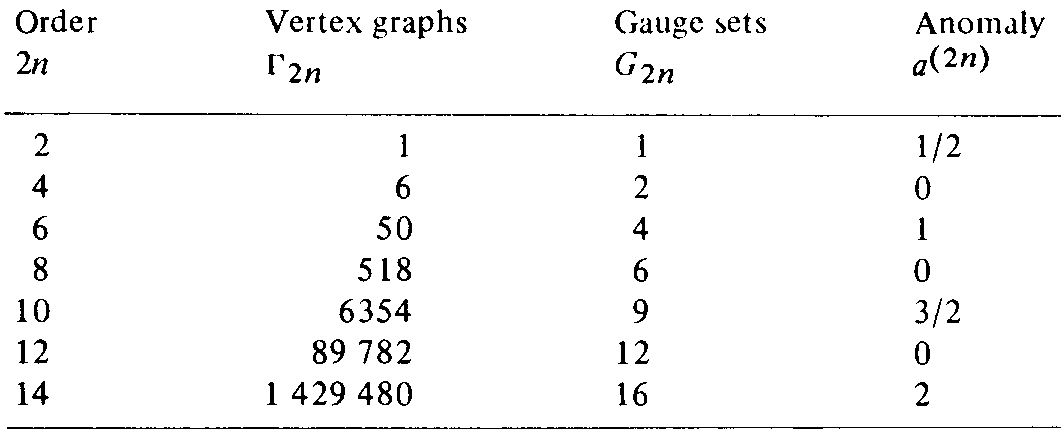
\includegraphics[width=0.80\textwidth]{../../figs/Cvit77bTab1}
\end{center}
{\scriptsize  %\caption{\label{Cvit77bTab1}
Comparison of the number of vertex diagrams without fermion loops, gauge
sets, and the ``gauge-set approximation''\footfullcite{Cvit77b} for the magnetic
moment in $2n$th order.
}
%%%%%%%%%%%%%%%%%%%%%%%%%%%%%%%%%%%%%%%%%%%%%%%%%%%%%%%%%%%
\end{frame}

\begin{frame}{Feynman's challenge, 12th Solvay Conference}
Is there any method of computing the anomalous moment of the
electron which, on first approximation, gives a fair approximation to the
$\alpha$ term and a crude one to $\alpha^2$; and when improved, increases
the accuracy of the $\alpha^2$ term, yielding a rough estimate to
$\alpha^3$ and beyond?\footfullcite{Feynman62}
\end{frame}

\begin{frame}{the unreasonable smallness of gauge sets}
%\label{sect:gaugeSetsSmall}

When the diagrams are grouped into
gauge sets,
a surprising thing happens; while the
finite part of each Feynman diagram is of order of 10 to 100,
and each one is UV and IR divergent, for $n=2,3$
every gauge set adds up to approximately
\[
		   \pm {1 \over 2} \left(\frac{\alpha}{\pi}\right)^n
\,,
\]
with the sign given by a simple empirical rule
\[
a_{kmm'} = (-1)^{m+m'}\frac{1}{2}
\] % ee{Cvit77b(5)}
\end{frame}


\begin{frame}{1977 (slightly wrong) four-loop prediction}
\begin{center}
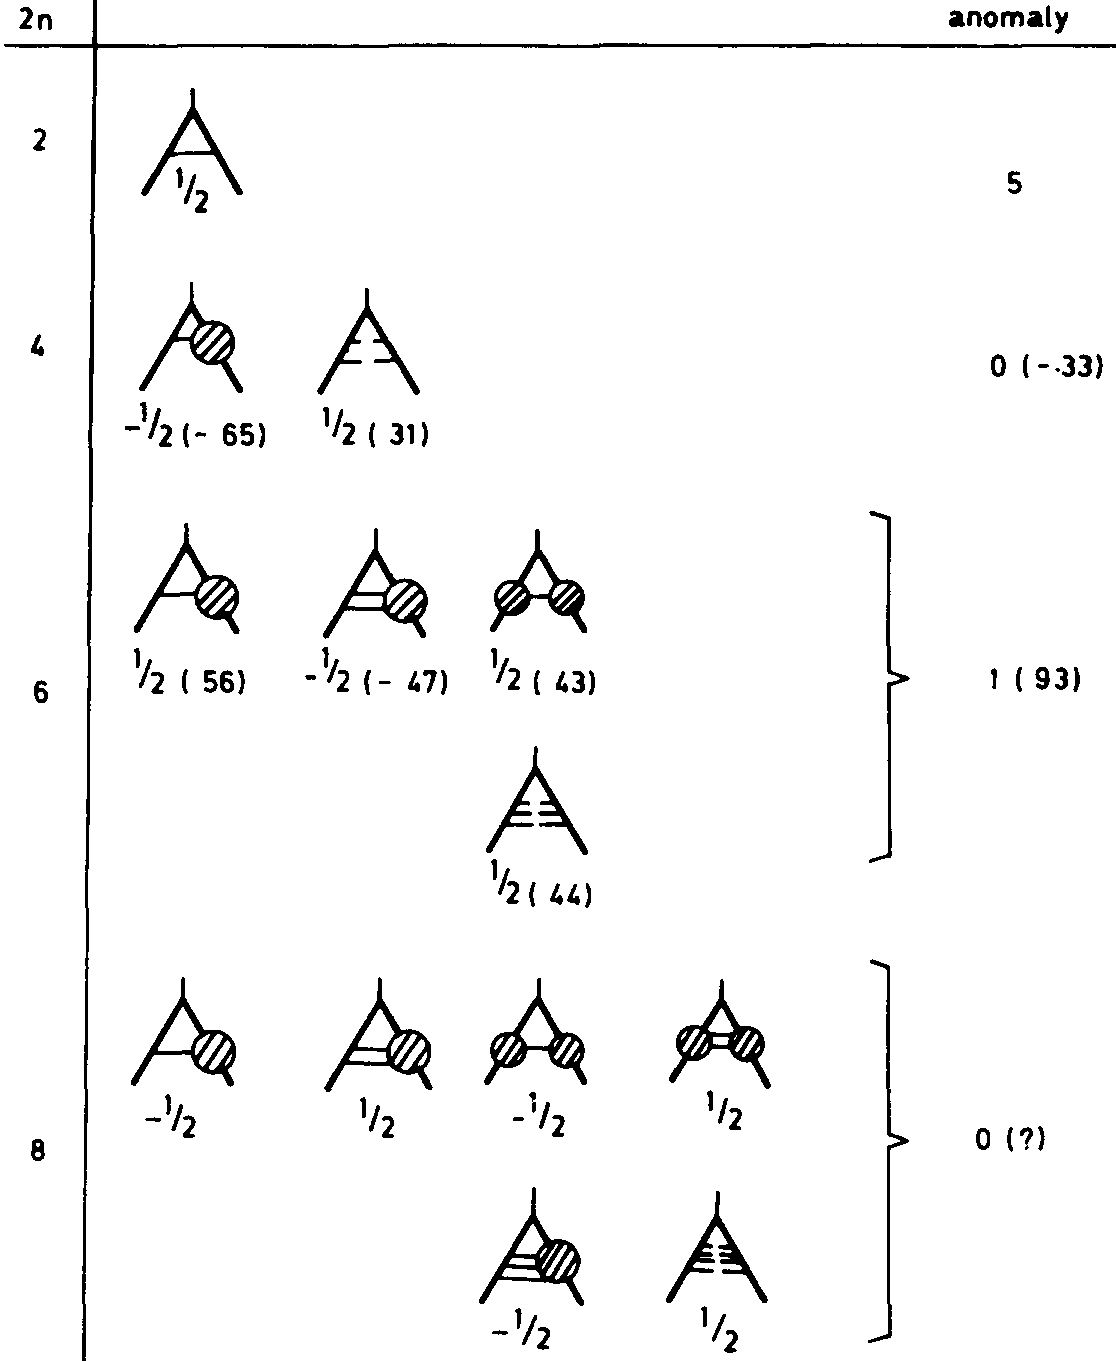
\includegraphics[width=0.50\textwidth]{Cvit77bFig3}
\end{center}

{\scriptsize  %\caption{\label{Cvit77bFig3}
new ``prediction'' : $a^{(8)}=-2$, rather than 0.
}
\end{frame}


\begin{frame}{an example of (slightly wrong) gauge-set approximation}
With prediction \(
a_{kmm'} = (-1)^{m+m'}\!/2
\) % ee{Cvit77b(5)}
, the ``zeroth'' order estimate of the electron
magnetic moment anomaly is given by the ``gauge-set
approximation,'' convergent and summable to all orders
\[ %\beq
a=\frac{1}{2}(g-2) =  \frac{1}{2} \frac{\alpha}{\pi}
                     \frac{1}
           {\left( 1 - \left(\frac{\alpha}{\pi}\right)^2
			\right)^2
		      } + \mbox{``corrections"}
\,.
\] %ee{Cvit77b(1)}
\end{frame}

\begin{frame}{request \#3}
\begin{center}
{\huge gauge invariance matters}
\end{center}
\end{frame}


\begin{frame}{forget Dyson}
most
colleagues believe that in 1952 Dyson\footfullcite{Dyson52} had  shown that the
QED perturbation expansion is an asymptotic series (for a discussion, see
Dunne and Schubert\footfullcite{DunSch06,HuTrSc17a}), in the sense that the $n$-th order
contribution should be exploding combinatorially
$$
{1 \over 2} (g-2) \approx
\cdots + n^n \left(\frac{\alpha}{\pi}\right)^n + \cdots
\,,
$$

contrast with my estimate
\[
{1 \over 2} (g-2) \approx
\cdots + \frac{n}{2}\left(\frac{\alpha}{\pi}\right)^{2n} + \cdots
\,.
\]
hence ``QED is finite'' claim
\end{frame}

\begin{frame}{request \#4 : prove that quenched QED is finite}
\begin{center}
{\huge any bound on a gauge set, exponential or slower, will do the trick!}
\end{center}
\end{frame}

\begin{frame}{so far facts ; next, speculation with Edwards and Schubert}
\begin{enumerate}
              \item
QED finiteness conjecture
              \item {\Large
bye bye, Feynman diagrams
                  }\textcolor{gray}{\small
              \item
worldline approach
                    }
\end{enumerate}
\end{frame}


\begin{frame}{bye bye, Feynman diagrams}
it's been a good ride, but there are way too many of you
\end{frame}

\begin{frame}{a fun fact}
the idea of how to avoid Feynman diagrams can be traced to 1950 Feynman
paper\footfullcite{Feynman50}, though it took a long time for it to gain
traction

\bigskip

by the time I explained the gauge set conjecture to
him in 1975, Feynman had forgotten all about it
\end{frame}

\begin{frame}{worldline path integral for the free scalar propagator}
propagator for the Euclidean
Klein-Gordon equation\footfullcite{Schubert12} is
\[ %\beq
D_0(x,x')=\bra{x}\frac{1}{-\Box +m^2}\ket{x'}
\,,
\] %ee{Schubert12(1.1)}
exponentiate the
denominator
\[ %\beq
D_0(x,x')=\int_0^\infty\!\!dT\,{e}^{-m^2T}\bra{x}e^{-T(-\Box)}\ket{x'}
\,,
\] %ee{Schubert12(1.4)}
replace the the $D$-dimensional Laplacian by a path integral
to obtain
\[ %\beq
D_0(x,x')=\int_0^\infty\!\!dT\,e^{-m^2T}
\int_{x(0)=x'}^{x(T)=x}\!\!\!\!\mathcal{D}x(\tau)\,
    e^{-\int_0^T\!\!d\tau \frac{1}{4}\dot{x}^2}
\,,
\] %ee{Schubert12(1.7)}
\end{frame}

\begin{frame}{worldline formula for charged propagator}
that emits and reabsorba $N$ photons as it
propagates%\footfullcite{AhBaSc16}

\medskip

Adding the QED
interaction terms leads to the Feynman's worldline path integral
representation\footfullcite{Feynman50} of the charged scalar propagator
in the presence of a background field $A(x)$,
\[ %\beq
D(x,x')=\int_0^\infty\!\!dT\,e^{-m^2T}
    \int_{x(0)=x'}^{x(T)=x}\!\!\mathcal{D}x(\tau)\,
            {e}^{-S_0-S_e-S_i}
\,,
\] %ee{AhBaSc16(1)}
where the suffix (0) indicates the free propagation
\[ %\beq
S_0 = \int_0^T\!\!d\tau \frac{1}{4}\dot{x}^2
\,,
\] %ee{Ahmadiniaz1}
(e) is the interaction of the charged scalar with the external field
\[ %\beq
S_e = -ie\int_0^T\!\!d\tau\,\dot{x}^\mu A_\mu(x(\tau))
\,,
\] %ee{Ahmadiniaz2}
\end{frame}

\begin{frame}{worldline formula for $N$-photon propagator}
and (i) are the virtual photons exchanged along the charged particle's
trajectory
\[ %\beq
S_i = \frac{e^2}{2}\int_0^T\!\!d\tau_1\int_0^T\!\!d\tau_2\,
      \dot{x}_1^\mu\,D_{\mu\nu}(x_1-x_2)\,\dot{x}_2^\nu
\,,
\] %ee{Ahmadiniaz3}
where $D_{\mu\nu} $ is the $x$-space photon propagator.

\medskip
The object of great interest to us is the internal virtual
photons term
\[ %\beq
\int_{x(0)=x'}^{x(T)=x}\!\!\mathcal{D}x(\tau)\,
            {e}^{-S_i}
=
\int_{x(0)=x'}^{x(T)=x}\!\!\mathcal{D}x(\tau)\,
            {e}^{-\frac{e^2}{2}\int_0^T\!\!d\tau_1\int_0^T\!\!d\tau_2\,
      \dot{x}_1^\mu\,D_{\mu\nu}(x_1-x_2)\,\dot{x}_2^\nu}
\] %ee{AhBaSc16(1)i}
expanded perturbatively in $\alpha/\pi$, this yields \\
the
usual $n!$ Feynman-parametric vertex diagrams
\end{frame}

\begin{frame}{worldline formalism}
however, the path integral is Gaussian in
$\dot{x}^\mu$, and if by integration by parts, $\dot{x}^\mu$ are
eliminated in favor of $x^\mu$, internal photons can be integrated over
directly, prior to an expansion in $(\alpha/\pi)^n$, and one gets
integrals in terms of

\begin{block}{$N$-photon propagators}
symmetrized sums over $N$ photons
\end{block}
and not the usual
Feynman graphs

\bigskip
each usual Feynman graph corresponds to one particular
permutation of internal photon insertions, and from that comes the
factorial growth in the number of graphs
\end{frame}

\begin{frame}{worldline formalism}
note : the worldline integrals are expressed
in terms of $N$-photon propagators, \\
the central ingredient that defines
the \textcolor{red!80!black}{gauge sets}

\bigskip
unlike the Feynman parameter integrals for individual vertex graphs, they are
independent of the ordering of the momenta $k_1,\ldots,k_N$; the worline formula
contains all $\approx N!$ ways of attaching the $N$ internal
photons to the charged particle propagator

\bigskip
worldline representation combines
\\
\textcolor{green!80!black}{combinatorially many} Feynman diagrams into

\medskip\hfill
a \textcolor{green!80!black}{{\Huge single}} integral

\end{frame}

\begin{frame}{worldline formalism}
In QED the $N$-photon propagator formulation combines into one integral
all Feynman graphs related by permutations of photon legs along fermion
lines, that is, it yield a \emph{single} integral for a gauge set
$kmm'$
\end{frame}

\begin{frame}{worldline formalism}
\begin{center}
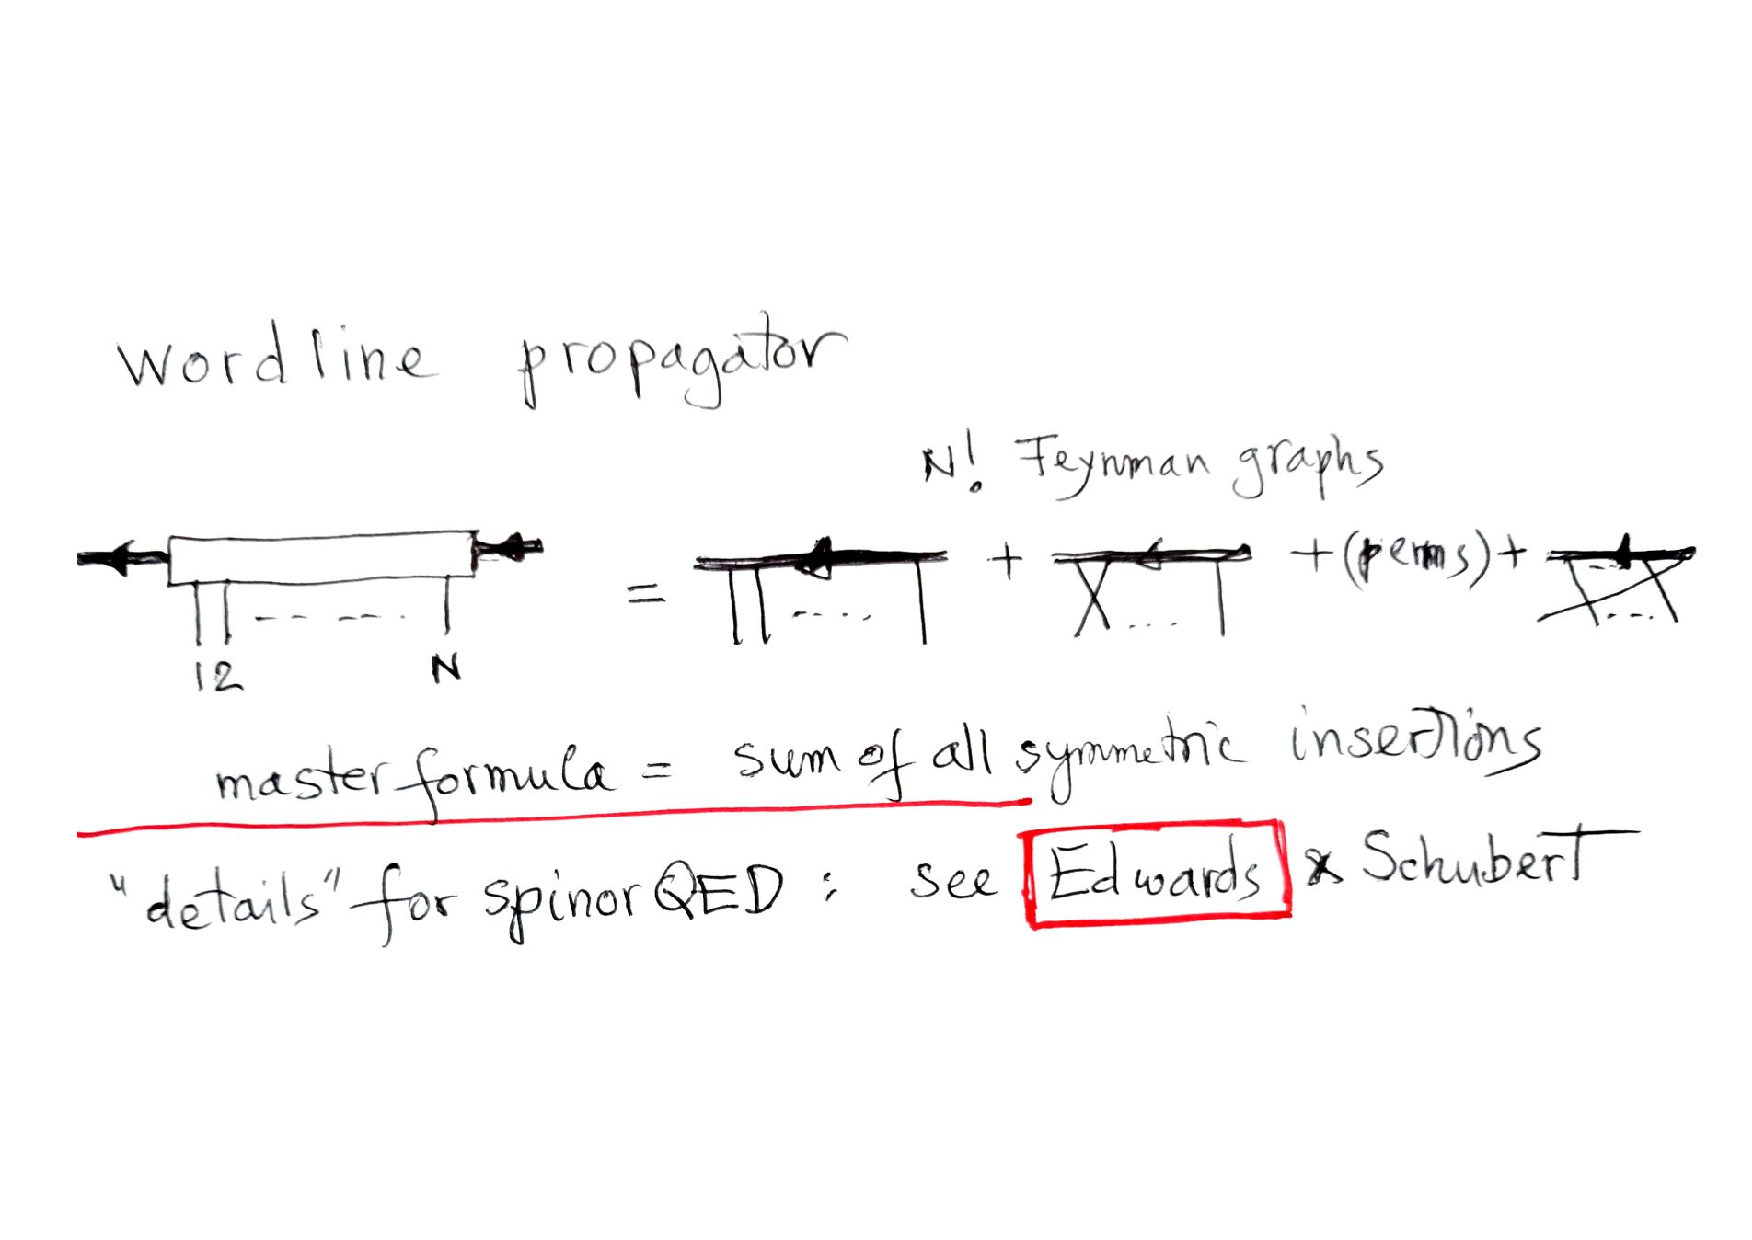
\includegraphics[width=0.90\textwidth]{worldlinProp}
\end{center}
\end{frame}
\begin{frame}{worldline formalism}
\begin{center}
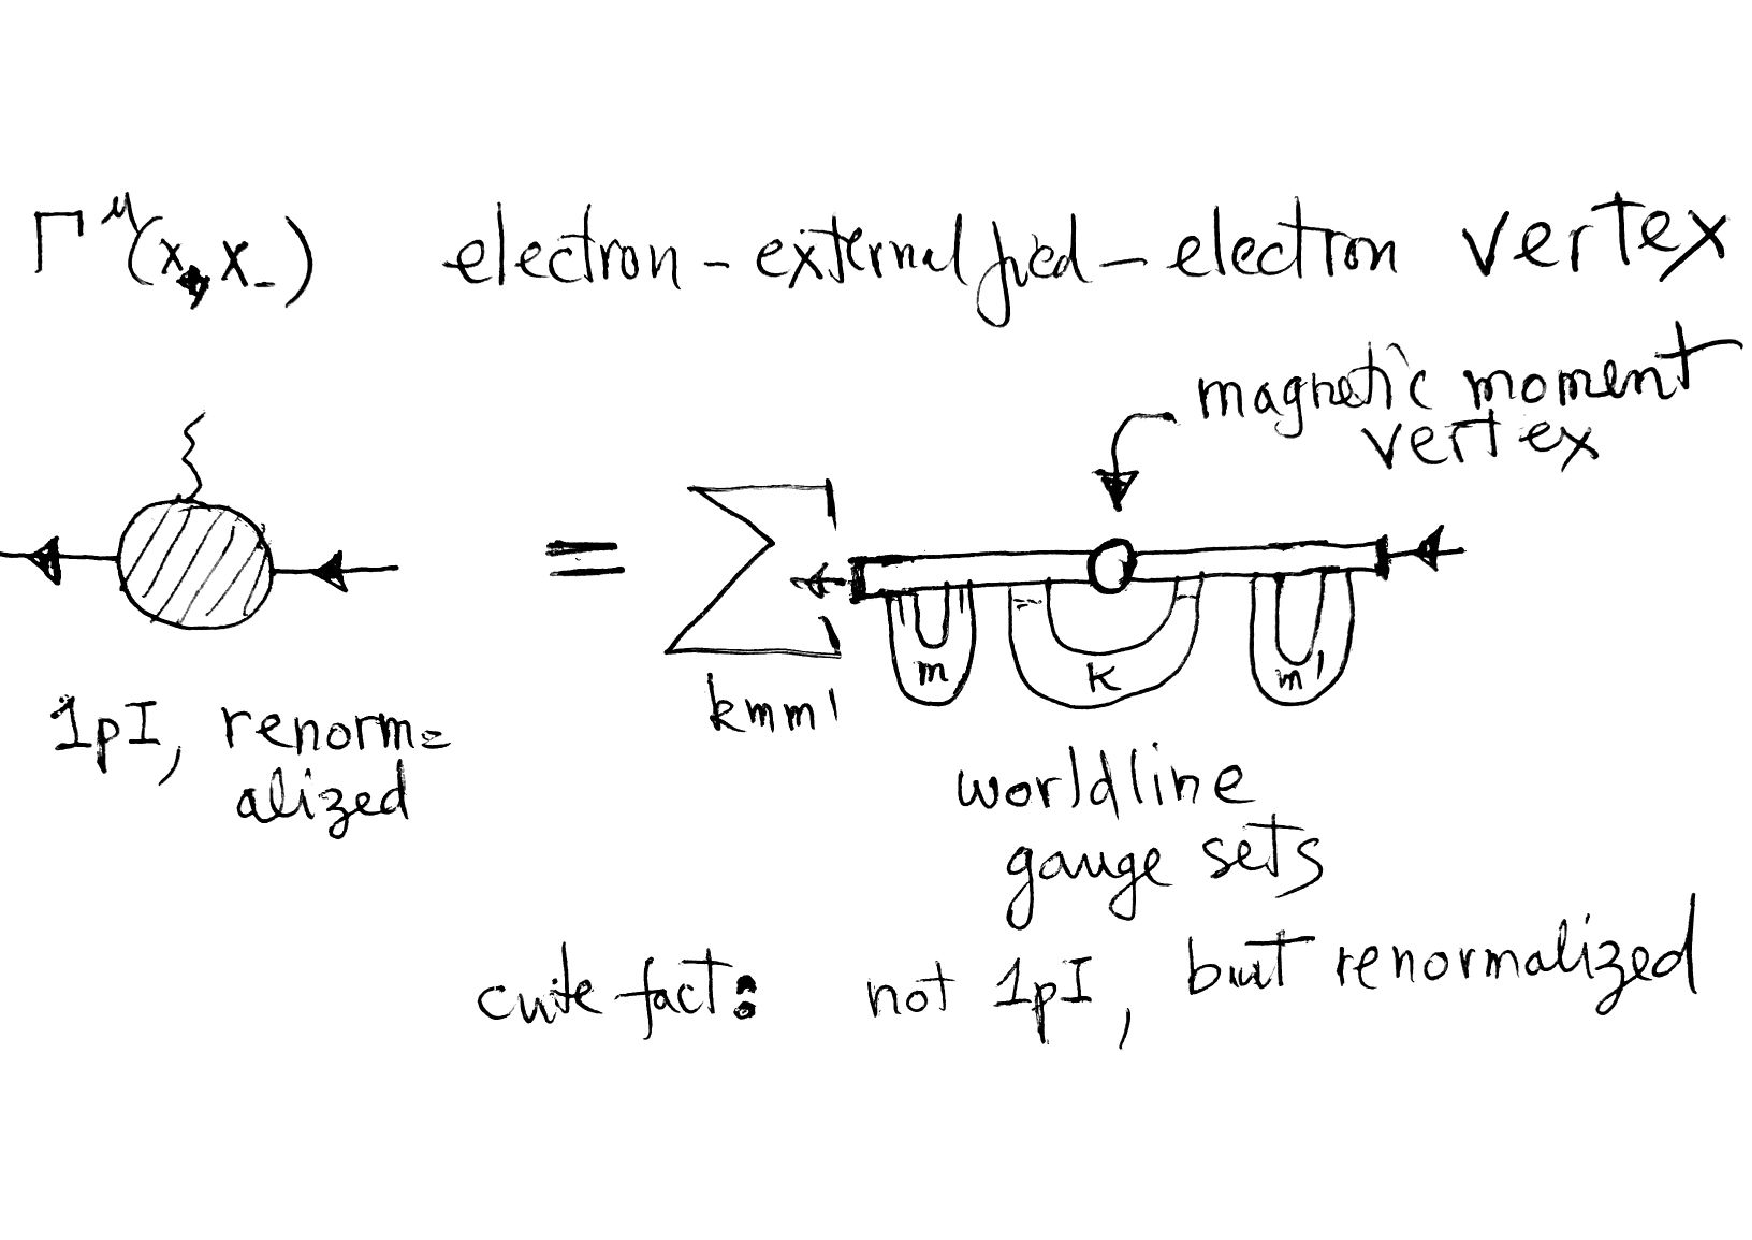
\includegraphics[width=0.90\textwidth]{worldlineGsets}
\end{center}
\end{frame}
\begin{frame}{worldline formalism}
\begin{center}
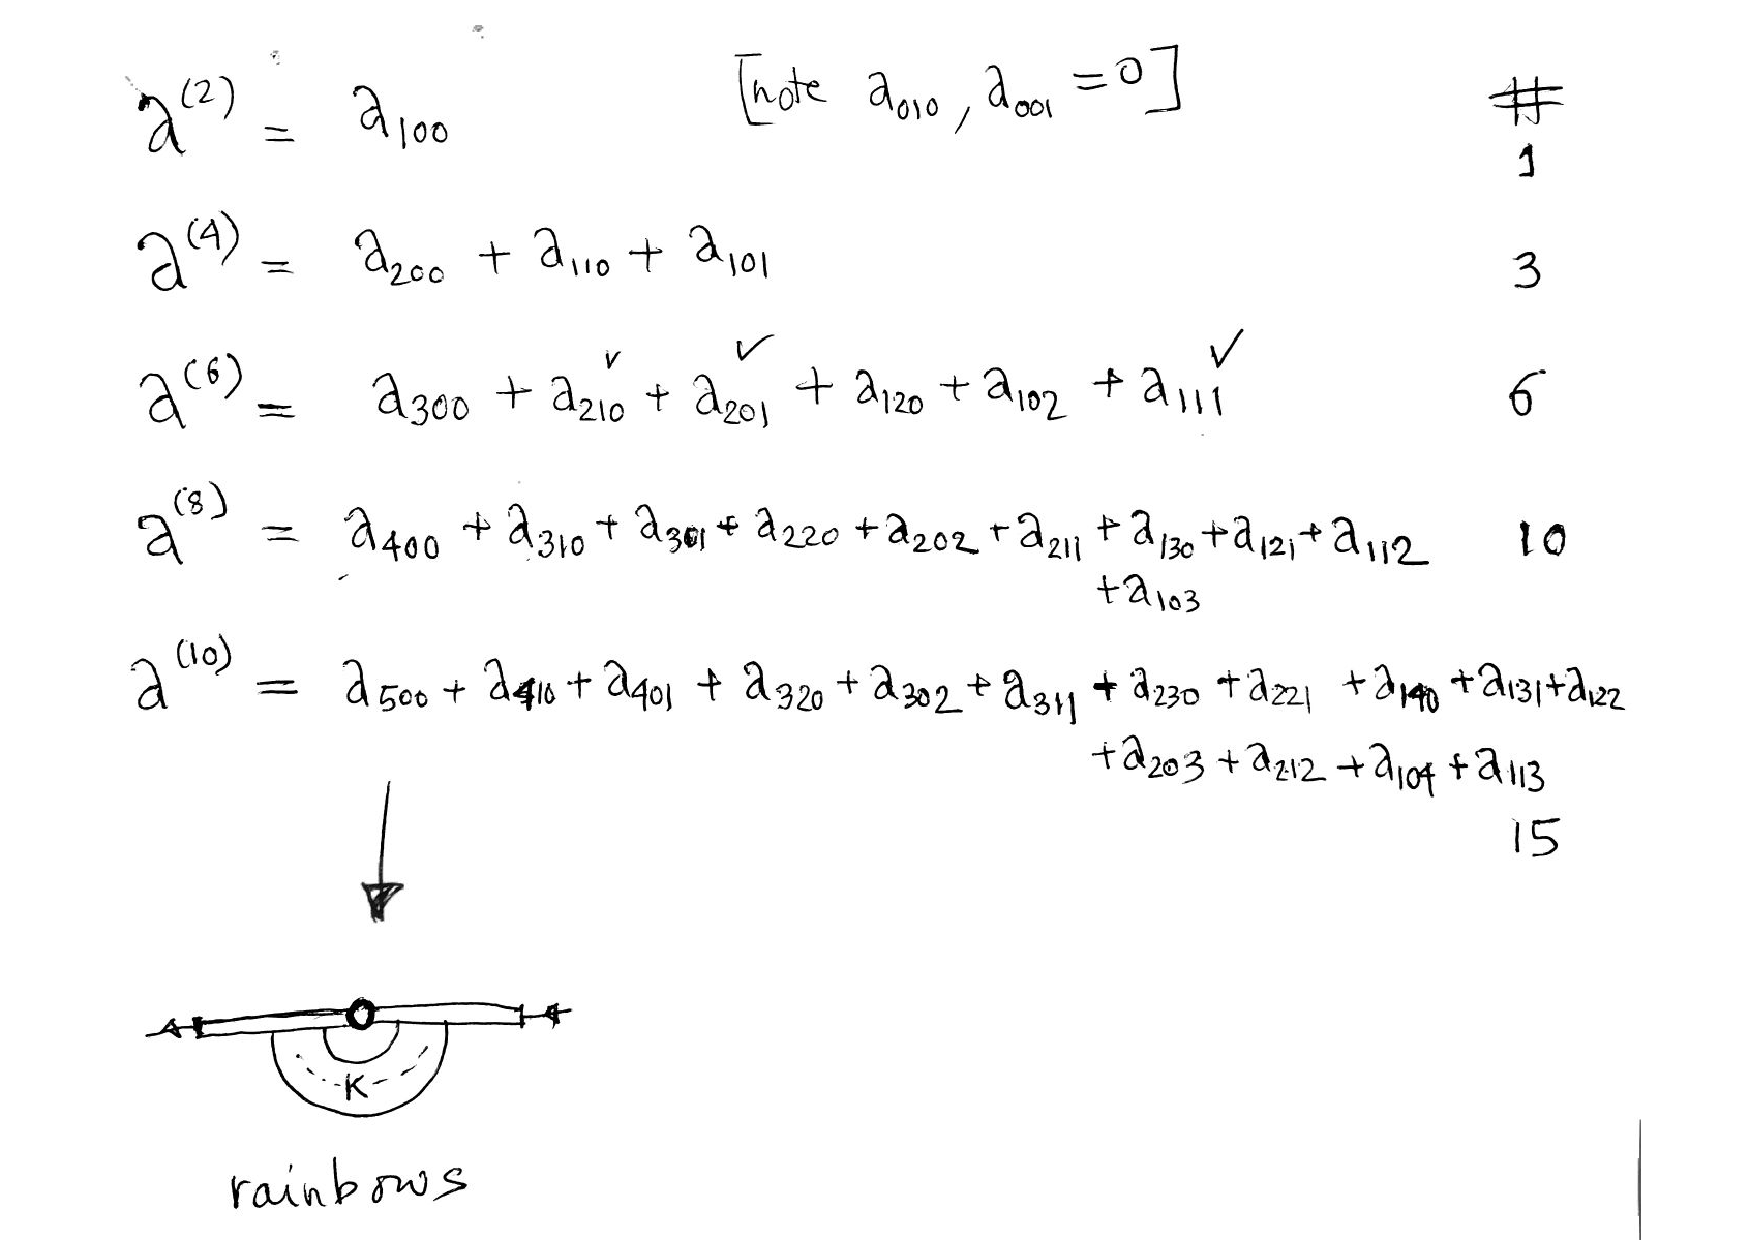
\includegraphics[width=0.50\textwidth]{gaugeSets}
\end{center}
\end{frame}
\begin{frame}{worldline formalism}
\begin{center}
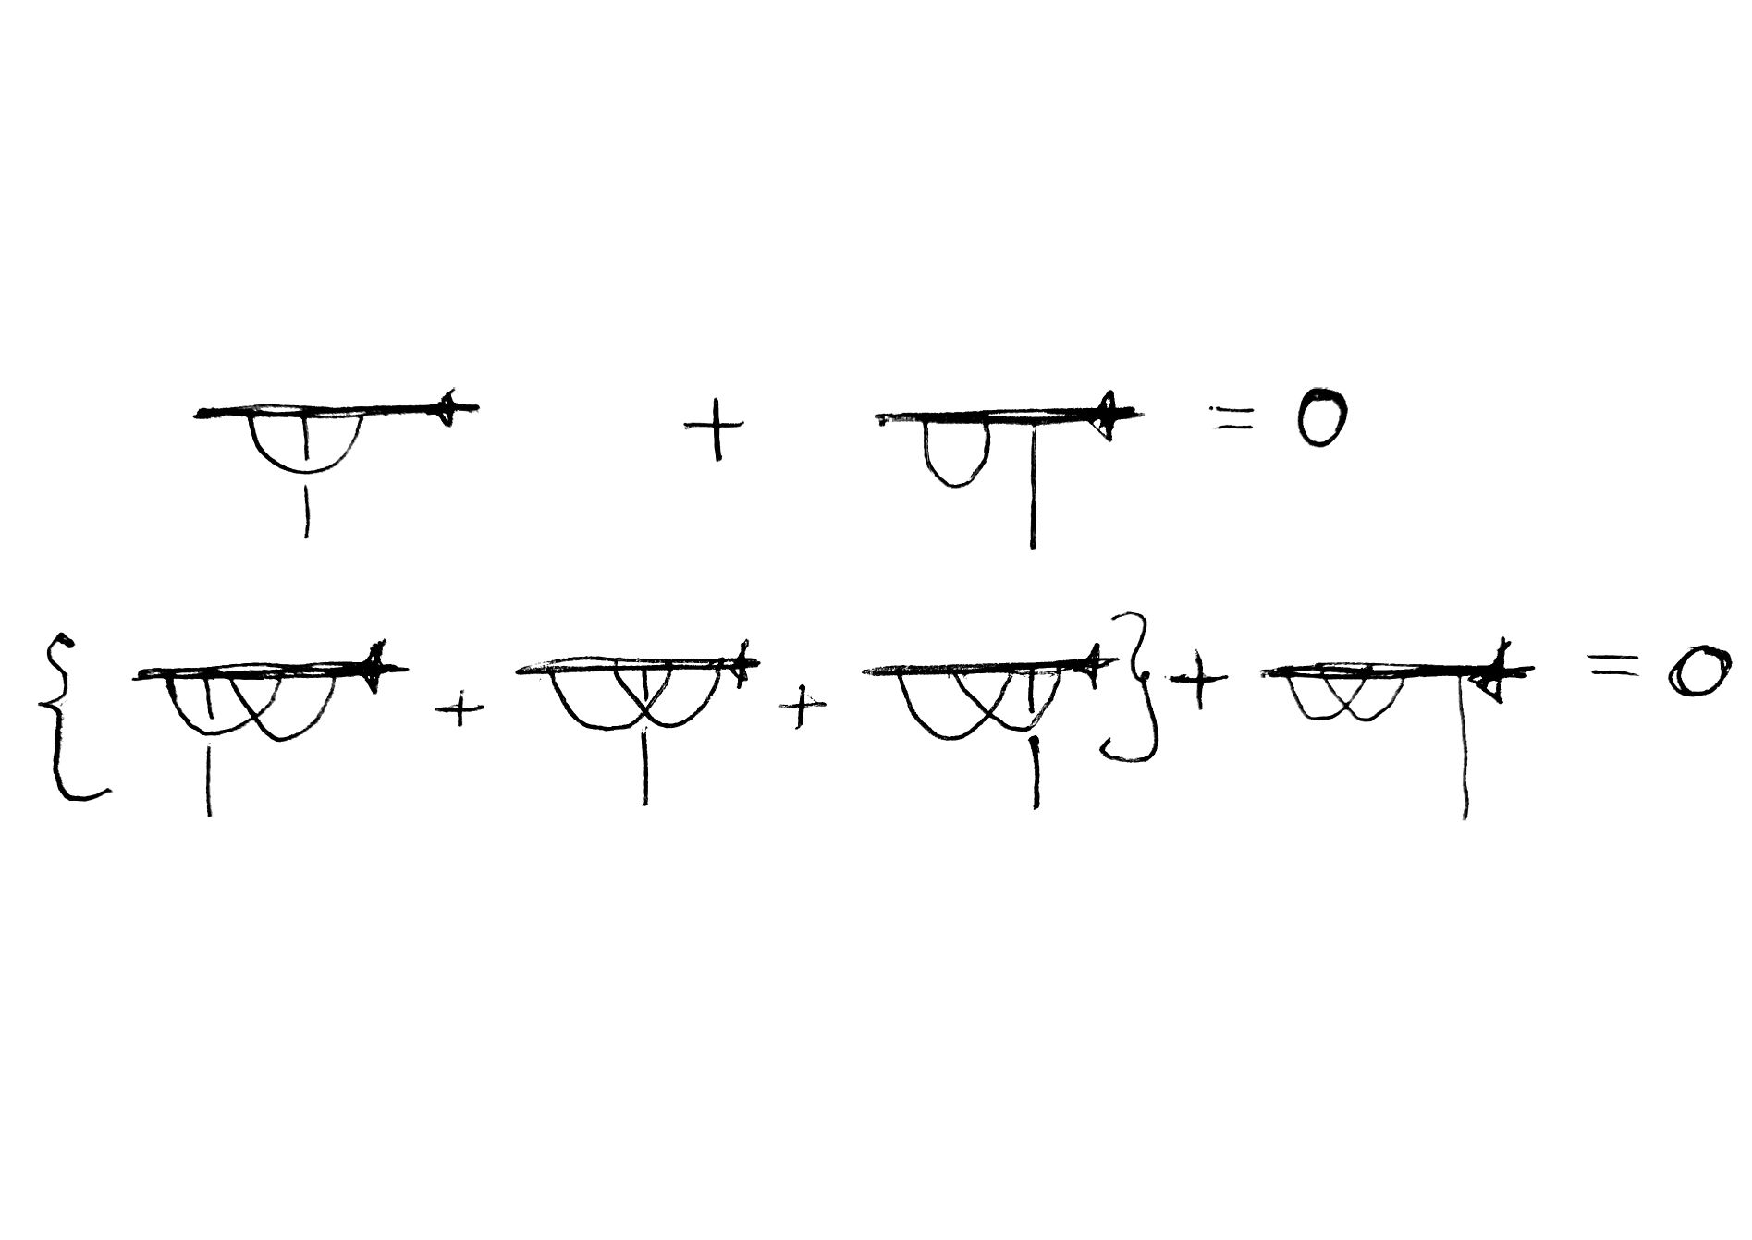
\includegraphics[width=0.90\textwidth]{WardIds}
\end{center}
\end{frame}
\begin{frame}{worldline formalism}
\begin{center}
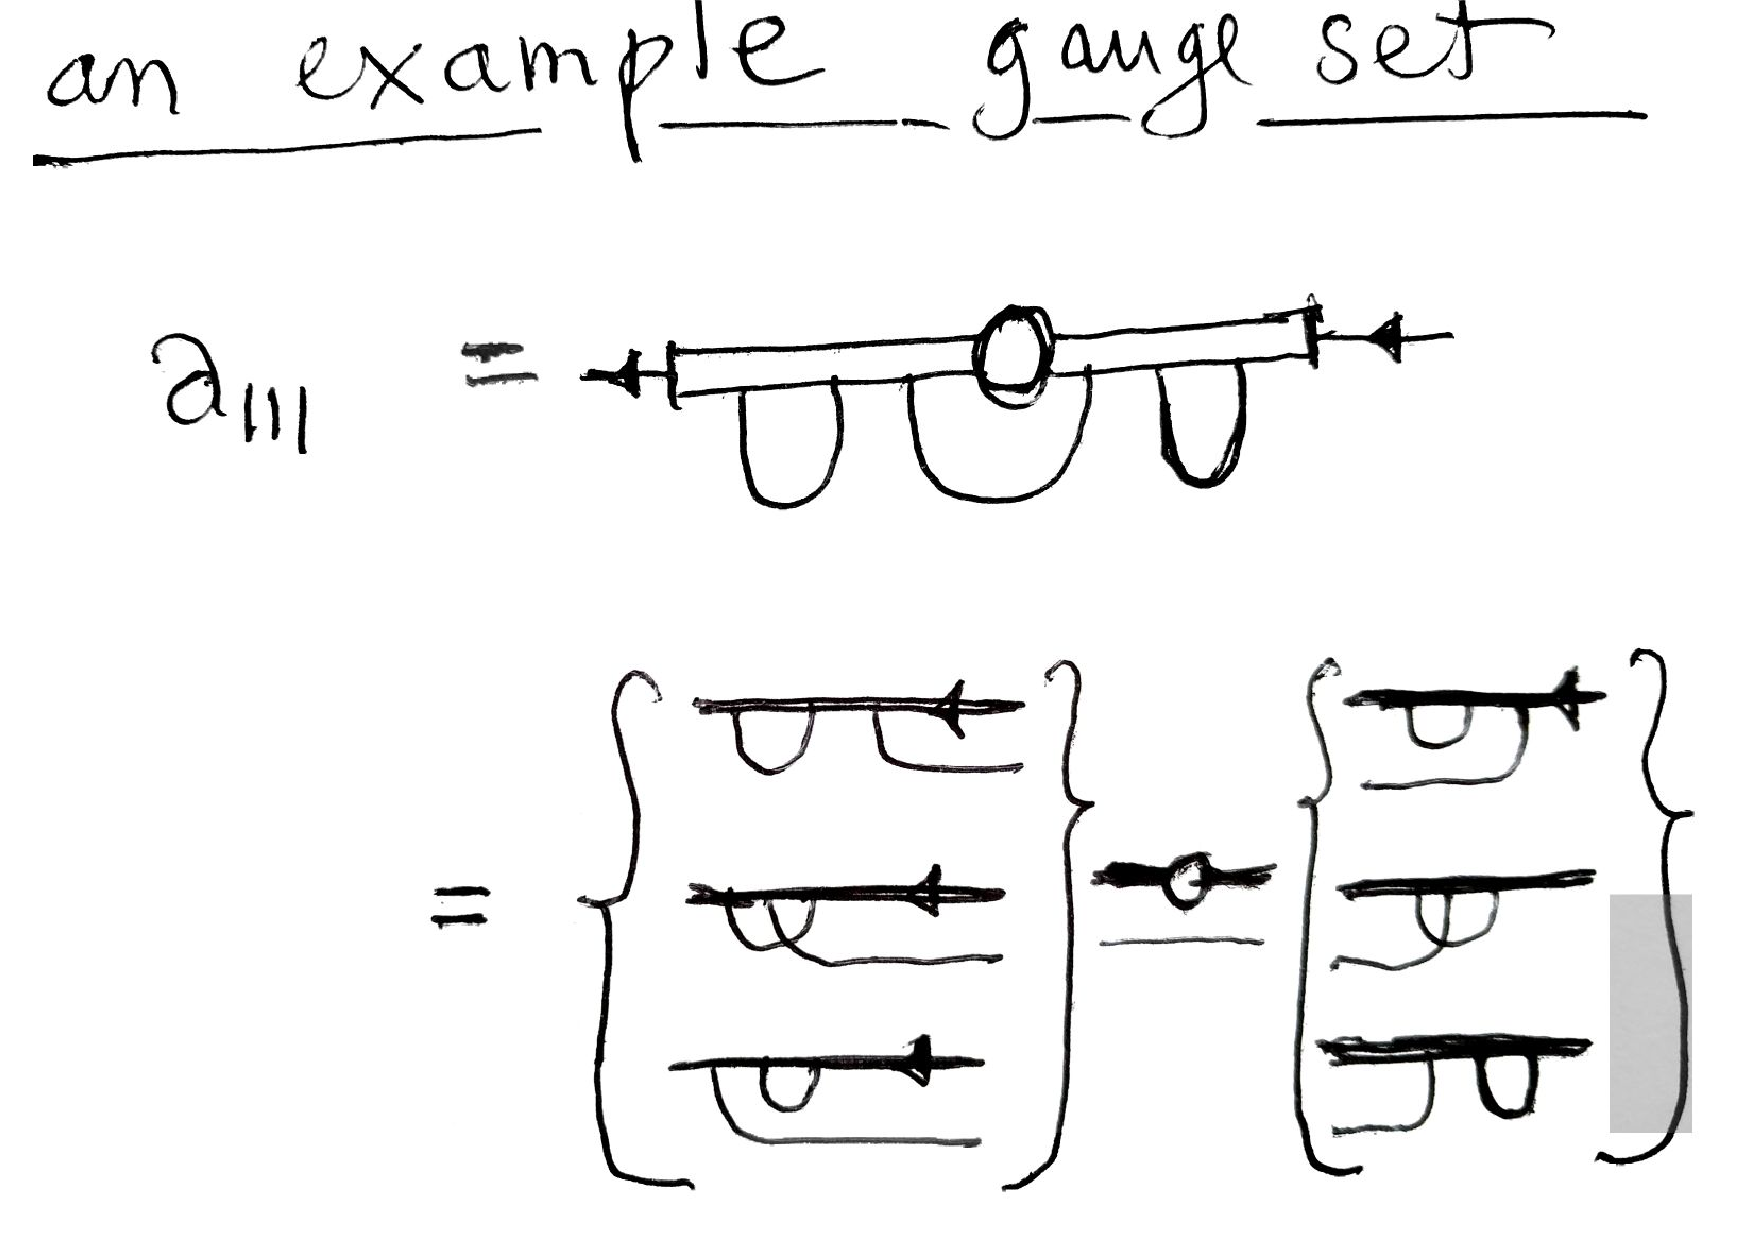
\includegraphics[width=0.90\textwidth]{a111a}
\end{center}
\end{frame}
\begin{frame}{worldline formalism}
\begin{center}
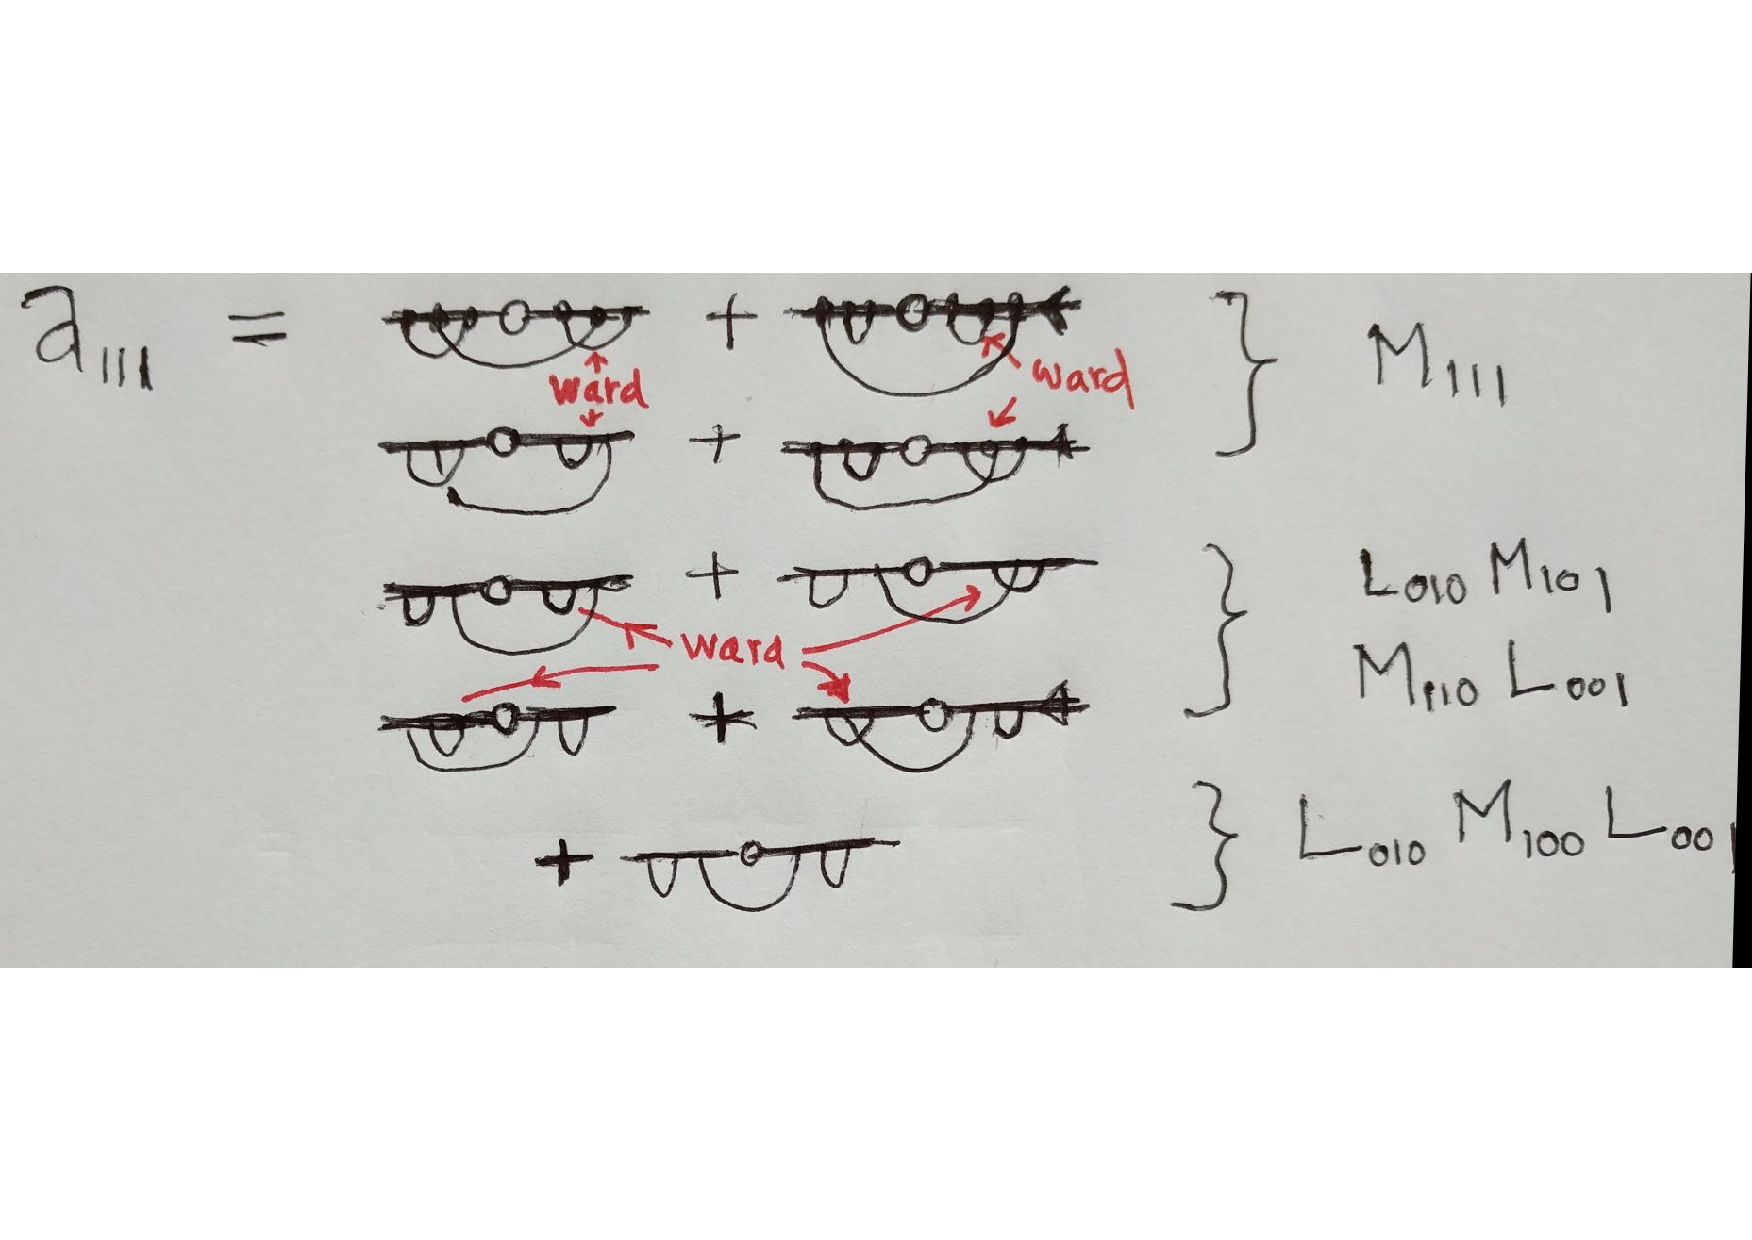
\includegraphics[width=0.90\textwidth]{a111b}
\end{center}
\end{frame}

\begin{frame}{summary}
\begin{enumerate}
              \item
a proof of the QED finiteness conjecture might be within reach

              \item
so might be methods for computing gauge invariant QFT sets without
recourse to Feynman diagrams

\end{enumerate}

\vfill
\bigskip\noindent{\scriptsize
you can download the current version of full notes here:
\HREF{http://chaosbook.org/~predrag/papers/finiteQED.pdf}
{ChaosBook.org/$\sim$predrag/papers/finiteQED.pdf}
\\The source code:
\HREF{https://GitHub.com/cvitanov/reducesymm/QFT}
{GitHub.com/cvitanov/reducesymm/QFT}
            }
\end{frame}



\end{document}
